%%% Local Variables:
%%% mode: latex
%%% TeX-master: t
%%% End:

\chapter{基于刻蚀-反应的光子晶体微球功能体系的研究}
\label{ch:etch-reaction}

\section{引言}

近年来,具有复杂结构及功能的纳米或微米颗粒在纳米材料、生物工程及有机电子学方面大放异彩。壳-核结构或多腔室结构带来了诸多新颖的性能及体系,包括等离子体增强\cite{Jin2010Multifunctional,Lim2011Highly}、能量传递系统\cite{Dimaio2008Controlling}、微反应器\cite{Peters2012From}、级联反应体系\cite{Vriezema2007Positional,Oers2014Cascade}等。为了制备这些具有复杂结构及组成的微材料,通常需要采用复杂的制备方法,例如逐步成核法\cite{Yec2012Synthetic}、逐层(LbL)生长法\cite{Son2013Systematic}、连续生物矿化法\cite{Shi2011Facile}以及两亲性分子自组装\cite{Zhang2014TemplateDirected,Tanaka2009Control,Koebe2012Crosslinked,Doh2004Photogenerated}以及微流控多相制备\cite{Ma2013CoreShell,Kim2011Generation}等方法。
这些方法主要为自下而上的制备方法,制备效率并不高,且容易造成颗粒尺寸不均一、多层之间偏心不匹配等问题\cite{Yec2012Synthetic}。且多数研究中仅局限于复杂结构的制备,而并未涉及对复杂结构的化学成分修饰及后续的功能体系设计。
同时,而自上而下对微材料的操作较自下而上的方法更为直接,
但目前较少有报道涉及自上而下的复杂结构制备方法。
因此,在制备复杂结构的微材料的同时赋予其空间上的化学复杂度对于功能材料的制备及研究具有非常重要的意义。前述介绍的光子晶体微球就是一种非常理想的功能平台。
由微流控液滴法制备的光子晶体微球具有可控的粒径及尺寸均一性;同时,这种微米级别的光子晶体微球在微纳尺度上包含了完整的光子晶体禁带特性,能够作为理想的微传感平台;此外,由纳米颗粒组装形成的内部孔道结构能够赋予光子晶体微球理想的物质流通特性。基于上述考虑,我们期望能够在光子晶体微球中实现立体的复杂结构制备及化学环境的调控,并通过上述结构实现更为复杂的功能体系。

与平面型光子晶体的图案化制备方法有所不同,光子晶体微球并不适用第~\ref{ch:photoactive}章中所采用的光掩膜光刻法,因为光子晶体微球的各向同性会造成紫外光透过球形的光子晶体结构而无法实现选择性的修饰目的。在对光子晶体微球进行HF刻蚀以制备反蛋白石光子晶体微球的过程中,我们意外地发现这种刻蚀过程需要一定的时间完成,而是在刻蚀过程中形成向内扩散的球形刻蚀边界。由于光子晶体微球球形表面的对称性及SiO\text{$_2$}微粒堆积的均匀性,这种刻蚀边界呈现很好的对称性与同心性。
在刻蚀进行的过程中,形成的刻蚀边界将光子晶体微球分为了两个部分,其中,在刻蚀边界之外的部分由于SiO\text{$_2$}的去除而形成了内部通透的反蛋白石结构,而内部的未刻蚀部分则是由SiO\text{$_2$}填充的复合模板。
利用内外部不同的通透性,结合化学反应对光子晶体的修饰方法,这里我们提出了一种基于可控刻蚀-反应的光子晶体微球修饰方法。
在本章中,我们利用琥珀酰亚胺(Suc)活化的羧基作为聚合物光子晶体中的功能基团来进行化学修饰。Suc活化的羧基能够与伯胺化合物在中性条件下发生酰胺化反应生成目标酰胺产物。
这种化学反应能够在中性条件下进行,同时只选择性针对氨基发生反应,在同等条件下不会与羟基、巯基等其余基团产生反应,因此能够很好的实现在醇类溶剂以及水相中的氨基修饰\cite{Pollak1980Enzyme}。同时,氨基的引入较易,在自然界中分布也十分广泛,使得可以被修饰的化合物具有极大的多样性,包括氨基亲疏水性小分子、氨基荧光分子乃至多肽或蛋白质等。本章中所设计的光子晶体微球的层次化修饰方法如图~\ref{fig:ch5-principle}。
\begin{figure}[htbp]
  \centering
  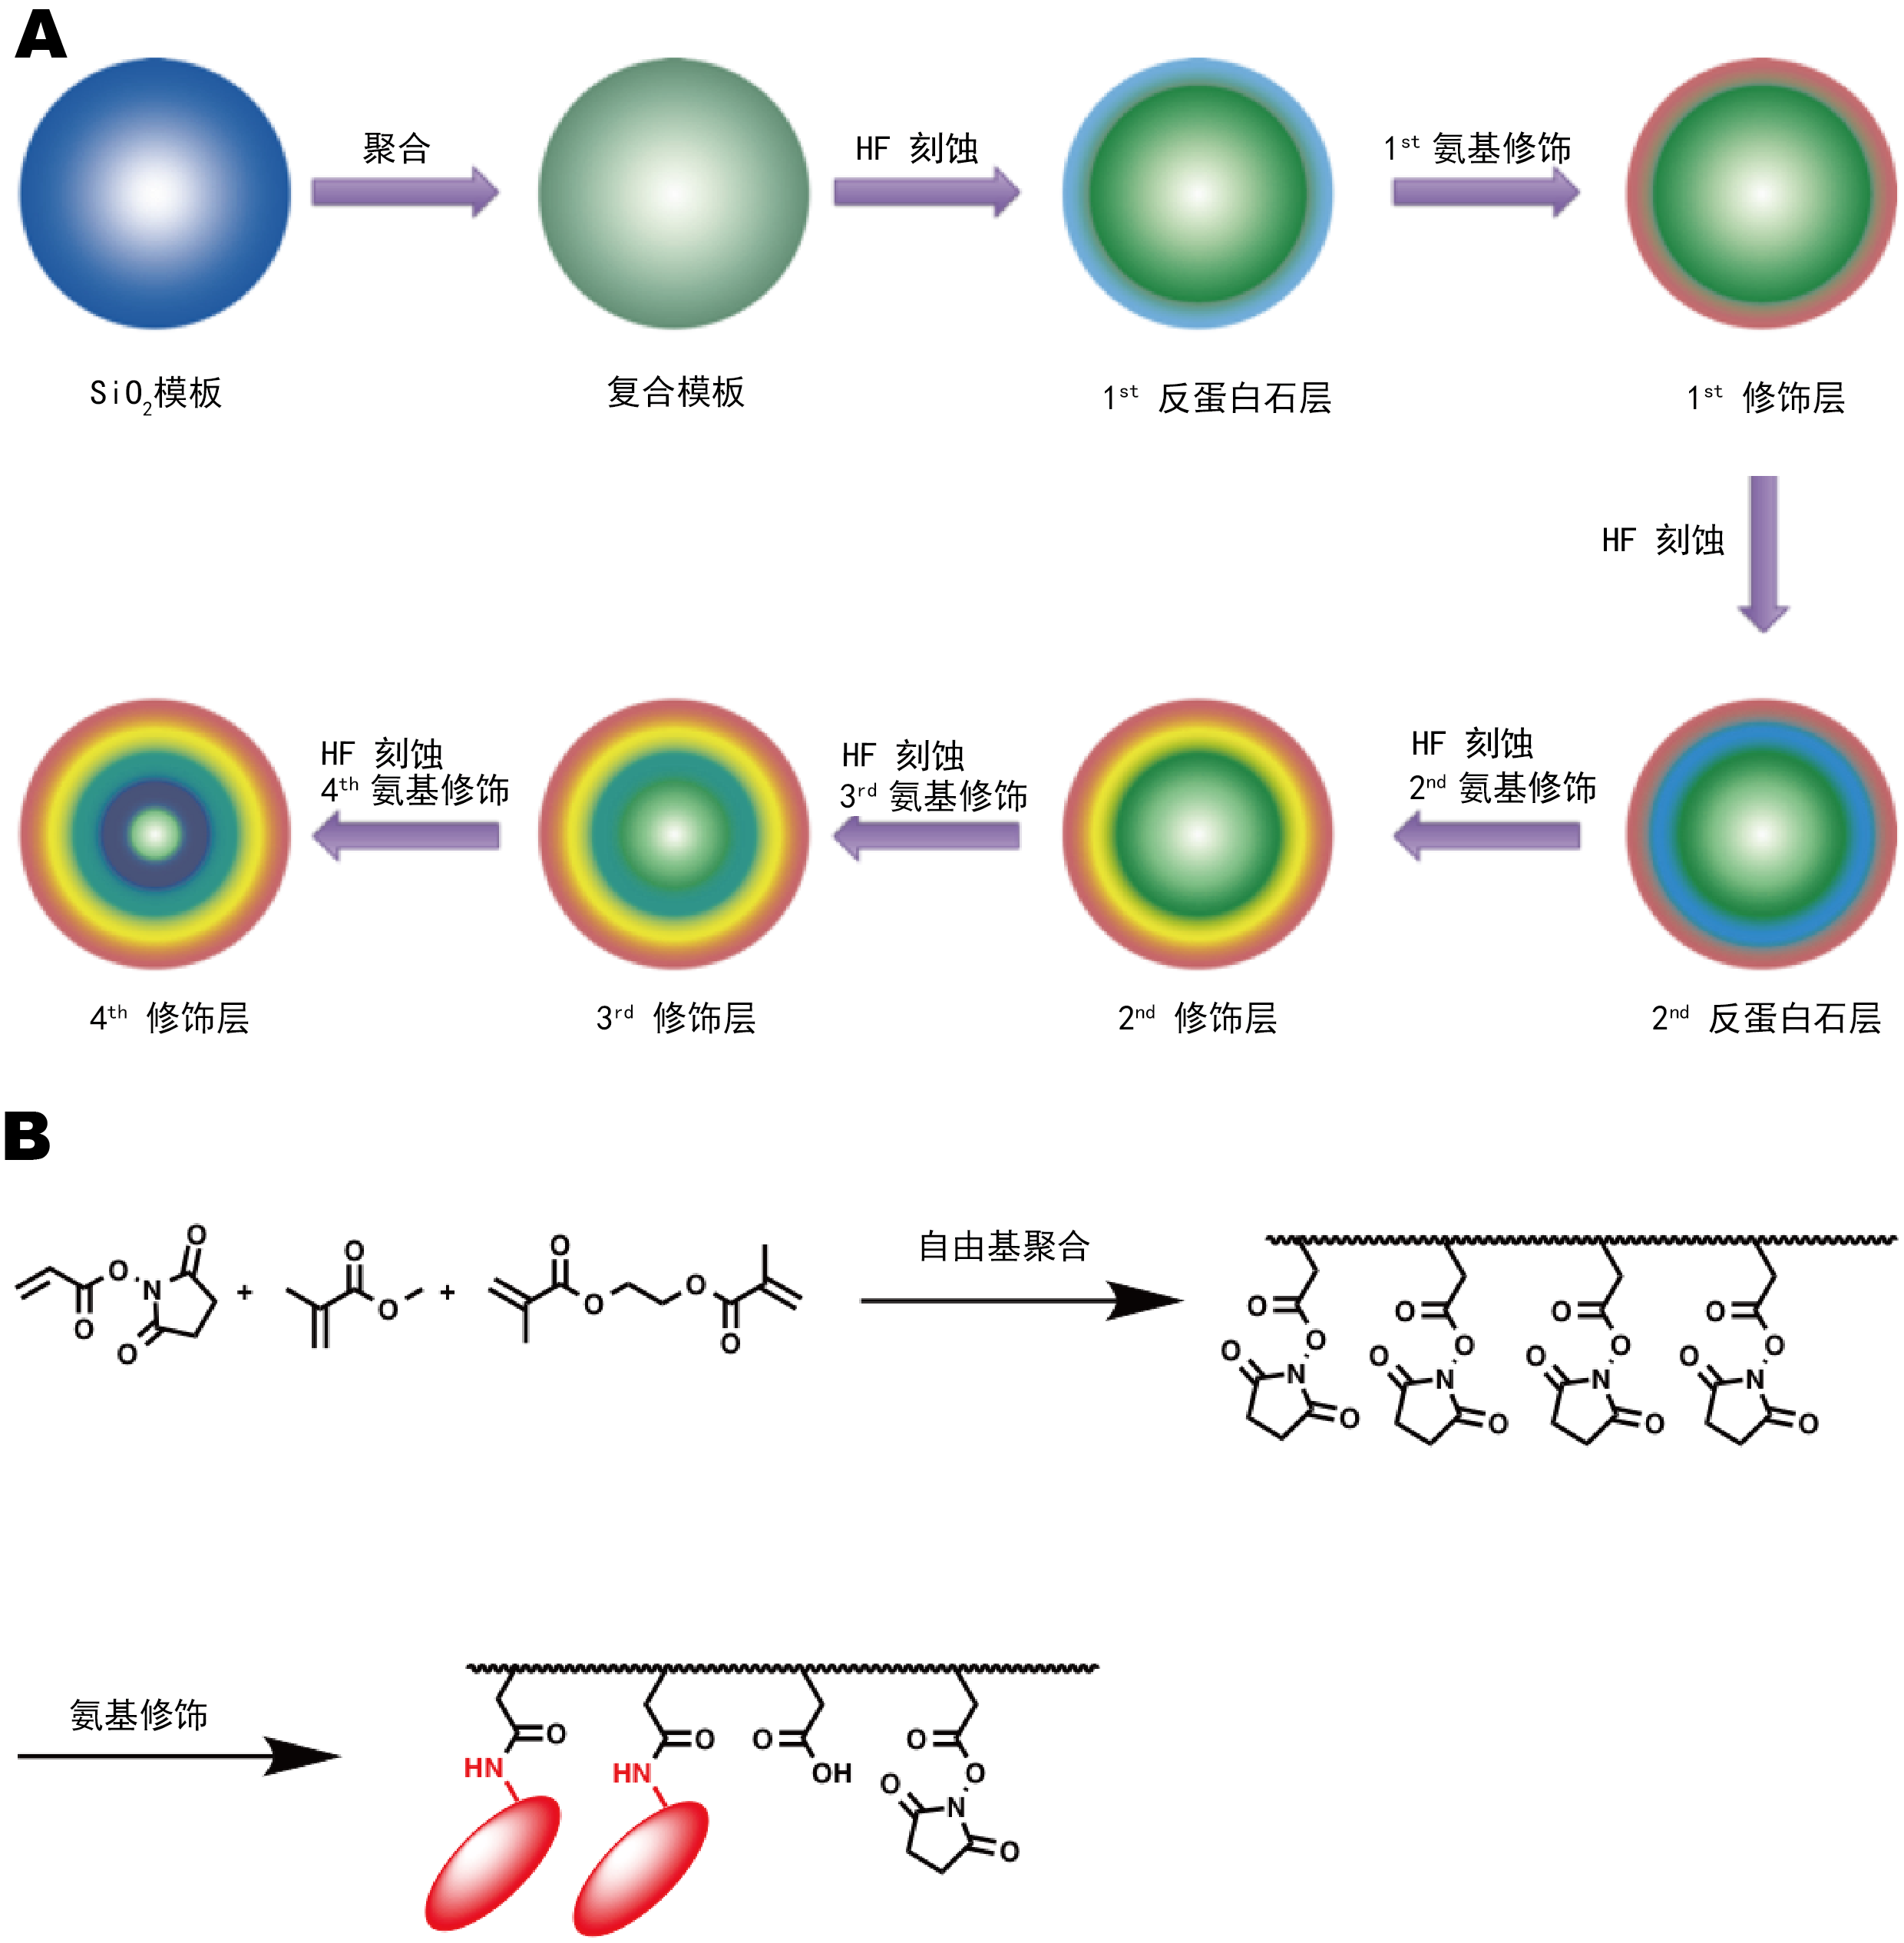
\includegraphics[width=\linewidth]{figures/ch5/ch5-principle.png}
  \caption{基于刻蚀-反应的光子晶体微球修饰方法示意图。A. 刻蚀-反应方法;B. Suc活化羧基高分子的修饰原理}
  \label{fig:ch5-principle}
\end{figure}

利用被刻蚀部分的反蛋白石光子的通透孔道结构与未刻蚀部分的封闭结构之间的差别来实现光子晶体微球的空间差异性修饰,最终形成具有多层同心结构的功能光子晶体微球。结合光子晶体微球的光学特性、内部孔道特性以及修饰后的空间化学复杂性,我们期望这种光子晶体材料能够发展为一系列复杂功能体系(图\ref{fig:scheme-3-2})。
\begin{figure}[htbp]
  \centering
  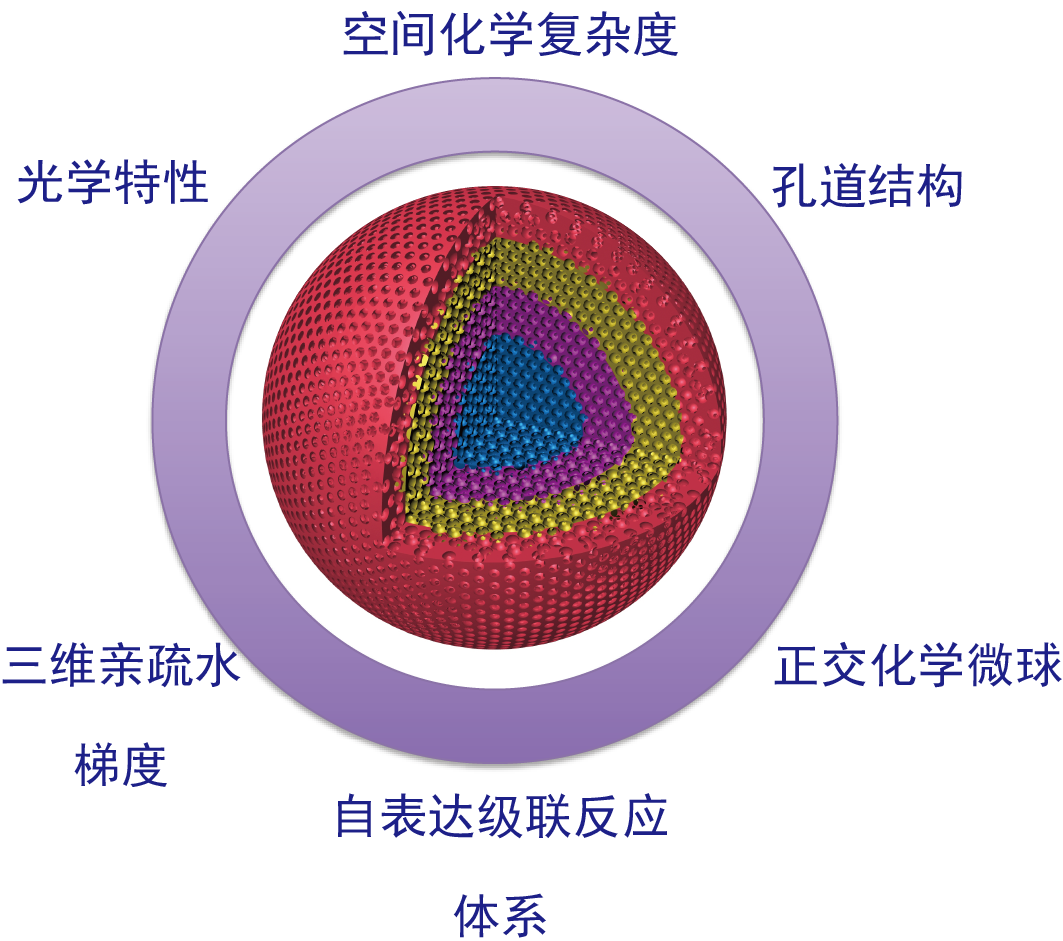
\includegraphics[width=0.6\linewidth]{figures/ch5/schem3-2.png}
  \caption{本章中多层次光子晶体微球的特性与拓展应用}
  \label{fig:scheme-3-2}
\end{figure}

\section{实验部分}
\label{sec:ch5-exp}

\subsection{实验材料与仪器}
本章中所使用的实验材料与仪器分别见
	表~\ref{tab:ch5-material}与~\ref{tab:ch5-instrument}。此前章节中已使用的材料这里不再赘述。

\begin{table}[htbp]
  \centering
  \caption{本章所用实验材料}
  \label{tab:ch5-material}
    \begin{tabularx}{\linewidth}{XXXX}
      \toprule[1.5pt]
      {\heiti 药品名称} & {\heiti 纯度} & {\heiti 来源} & {\heiti 处理方法}\\
      \midrule[1pt]
      二甲亚砜(DMSO) & 分析纯 & 国药集团化学试剂有限公司 & 分子筛干燥\\
      丙酮 & 分析纯 & 国药集团化学试剂有限公司 & 分子筛干燥\\
      乙二醇 & 分析纯 & 国药集团化学试剂有限公司 & 分子筛干燥\\
      乙二胺 & 分析纯 & 国药集团化学试剂有限公司 & 直接使用\\
      罗丹明B(RhB)& 98\% & Alfa Aesar & 直接使用\\
      3-溴丙胺氢溴酸盐 & 98\% & Alfa Aesar & 直接使用\\
      NaN\text{$_3$} & 98\% & Alfa Aesar & 直接使用\\
      环庚烯 & 98\% & J\&K Chemical & 直接使用\\
      叔丁醇钾 & 98\% & J\&K Chemical & 直接使用\\
      1,8-二氮杂二环十一碳-7-烯(DBU) & 98\% & J\&K Chemical & 直接使用\\
      溶剂绿7(cascade blue)& 98\% & J\&K Chemical & 直接使用\\
      溴乙酸乙酯& 98\% & Alfa Aesar & 直接使用\\
      N,N-二异丙基乙胺(DIEA)& 98\% & J\&K Chemical & 直接使用\\
      1-乙基-(3-二甲基氨基丙基)碳酰二亚胺 & 98\% & Alfa Aesar & 直接使用\\
      胆碱氧化酶(ChOx)& >25 U/mg & Sigma-Aldrich & 直接使用\\
      辣根过氧化酶 & >500 U/mg & Sigma-Aldrich & 直接使用\\
      丽斯胺罗丹明 B 酰氯 & 98 \% & Sigma-Aldrich & 直接使用\\
      异硫氰荧光素(FITC) & 98 \% & Sigma-Aldrich & 直接使用\\
      N,N-二甲基乙二胺(DMEA) & 98 \% & Alfa-Aesar & 直接使用\\
      十二胺(DDA) & 98 \% & Alfa-Aesar & 直接使用\\
      2,2’-联氮双 (3-乙基苯并噻唑啉 -6-磺酸) 二铵盐(ABTS) & 98\% & J\&K Chemical &直接使用\\
      卢米诺 & 98\% & J\&K Chemical &直接使用\\
      \bottomrule[1.5pt]
    \end{tabularx}
\end{table}

\begin{table}[htbp]
  \centering
  \caption{本章所用仪器}
  \label{tab:ch5-instrument}
    \begin{tabularx}{\linewidth}{XXX}
      \toprule[1.5pt]
      {\heiti 仪器名称} & {\heiti 仪器规格} & {\heiti 厂家} \\
      \midrule[1pt]
      反射光纤光谱仪 & USB2000 & OceanOptics\\
      场发射扫描电子显微镜(SEM) & LEO-1503 & Bruker\\
      傅里叶变换红外光谱仪(FTIR)& PE 2000 & Perkin-Elmer\\
      核磁共振仪(NMR) & ECA 300 &JEOL\\
      电喷雾质谱仪(ESI) &Esquire-LC &Bruker\\
      接触角测定仪 & OCA 20 &Dataphysics\\
      激光共聚焦荧光显微镜(CLMS) &N-SIM &Nikon\\
      \bottomrule[1.5pt]
    \end{tabularx}
\end{table}

\subsection{相关化合物的合成}
1. Suc活化羧基功能单体的制备
由琥珀酰亚胺活化的单体的制备过程如图~\ref{fig:suc-monomer}
\begin{figure}[htbp]
  \centering
  
\includegraphics[width=0.75\linewidth]{figures/ch5/ch5-NAS.png}
  \caption{Suc活化羧基功能单体的制备}
  \label{fig:suc-monomer}
\end{figure}

化合物10(NSA):将3.45 g(30.0 mmol, 1 eqiv)NHS、4.6 mL TEA溶解于30 mL CH\text{$_2$}Cl\text{$_2$}中。在冰浴搅拌的同时,用恒压滴液漏斗向烧瓶内滴入2.68 mL (33.0 mmol,1.1 eqiv)的丙烯酰氯。随着反应的进行,溶液中逐渐产生白色沉淀。反应进行2 h后将沉淀过滤去除。有机相用饱和NaCl溶液洗涤2次,干燥浓缩后用纯CH\text{$_2$}Cl\text{$_2$}展开剂进行柱层析提纯。最终获得白色晶体(3.84 g, 75.9\%)。
化合物9:2,5-二氧代吡咯烷基丙烯酸酯,\text{$^1$}H-NMR(300 MHz,CDCl\text{$_3$}): \text{$\delta$} 2.62 (s, 4H, CH\text{$_2$}CH\text{$_2$}), 5.83 (m, CH(H)=), 6.10 (d, CH=), 6.39 (m, CH(H)=)。 ESI-MS: 192.1 [M+Na]\text{$^+$}。

2. 荧光标记分子的合成

本章中涉及到多种荧光标记分子的合成,分别叙述如下。

氨基修饰的罗丹明B标记分子(化合物11)的合成路线如图~\ref{fig:amine-RhB}所示。
\begin{figure}[htbp]
  \centering
  
\includegraphics[width=0.95\linewidth]{figures/ch5/ch5-RhB-An.png}
  \caption{氨基修饰的罗丹明B标记分子的合成}
  \label{fig:amine-RhB}
\end{figure}

化合物11:将245 mg (0.5 mmol, 1 eqiv)罗丹明B溶解于60 mL乙醇中,在搅拌过程中加入1.48 g (20 mmol, 40 equiv)乙二胺。反应溶液回流12 h。随着反应的进行,溶液的深红色逐渐减弱并褪为橙黄色。反应液冷却后,将乙醇旋蒸除去,向残余液体中加入 1 M HCl溶液将残余乙二胺中和。随后用1 M NaOH溶液将混合溶液的调节至pH=10,并用30 mL CH\text{$_2$}Cl\text{$_2$}萃取三次。合并的有机相干燥浓缩后用50:1 CH\text{$_2$}Cl\text{$_2$}:MeOH展开剂在碱性氧化铝层析柱中提纯产物,得到白色至粉色固体(197 mg,72.0\%)。
化合物11:氨乙基罗丹明B内酰胺,\text{$^1$}H-NMR(300 MHz,CDCl\text{$_3$}): \text{$\delta$} 1.18 (m, 12H, CH\text{$_3$}), 2.40 (t, 2H, CH\text{$_2$}-NH\text{$_2$}), 3.20 (t, 2H, CONH-CH\text{$_2$}), 3.36 (q, 8H, CH\text{$_2$}CH\text{$_3$}), 6.25-7.90 (m, 10H, Ph-H)。ESI-MS: 485.3 [M+H]\text{$^+$}。

正交化学体系中涉及的相关分子的合成见图~\ref{fig:synth-orthognal}。
\begin{figure}[htbp]
  \centering
  
\includegraphics[width=\linewidth]{figures/ch5/synth-orthognal.png}
  \caption{正交化学体系中设计的相关分子的合成}
  \label{fig:synth-orthognal}
\end{figure}
% 其中,分子12-1的合成可以参考文献\onlinecite{Reese1975Preparation},

化合物12:将5.47 g(35.5 mmol, 1 eqiv)3-溴丙胺氢溴酸盐与3.25 g (50.0 mmol,1.4 eqiv)NaN\text{$_3$}溶于20 mL去离子水中,在回流条件下反应20 h。将反应液冷却后浓缩至5 mL,在冰浴条件下加入KOH将pH值调节至14。用50 mL乙醚萃取三次,将合并的有机相干燥旋蒸,得到无色具有胺气味的液体(3.04 g, 86.3 \%)。
化合物12:3-叠氮-1-丙胺,\text{$^1$}H-NMR(300 MHz,CDCl\text{$_3$}): \text{$\delta$} 1.84 (m, 2H, C-CH\text{$_2$}-C), 2.05 (s, 2H, NH\text{$_2$}), 2.86 (t, 2H, N\text{$_3$}-CH\text{$_2$}), 3.35 (t, 2H, NH\text{$_2$}-CH\text{$_2$})。ESI-MS:101.2 [M+H]\text{$^+$}。

化合物13:将3.65 g(38.0 mmol, 1 eqiv)环庚烯与8.52 g(76.0 mmol, 2 eqiv)叔丁醇钾分散于20 mL干燥的环己烷中。在氮气氛围下冰盐浴搅拌30 min,随后在冰盐浴中向悬浮液中滴加4.9 mL(57.0 mmol, 1.5 eqiv)溴仿,滴加在30 min内完成。随着溴仿的加入,反应混合物从白色变为棕色。冰盐浴反应2 h后继续在室温条件下进行。24 h后向反应混合物中加入100 mL去离子水淬灭反应,并用1M HCl溶液将反应液调节至中性。将有机相分离,并用环己烷萃取水相2次。合并的有机相干燥浓缩后用纯石油醚作为展开剂进行柱层析提纯。得到无色具有芳香气味的液体(8.65 g,83.2\%)。
化合物13:8,8-二溴环[5.0.1]辛烷,\text{$^1$}H-NMR(300 MHz,CDCl\text{$_3$}): \text{$\delta$} 1.05-1.22 (m, 3H), 1.28-1.40 (m, 2H), 1.62-1.72 (m, 2H), 1.76-1.92 (m, 3H), 2.25-2,28 (m, 2H)。ESI-MS:266.5 [M+H]\text{$^+$}。

化合物14:将13 mL (233 mmol,20 eqiv)无水乙二醇与7.24 g(34.9 mmol,3 eqiv)无水高氯酸银分散于10 mL无水丙酮中。在避光条件下常温搅拌,并同时滴加3.12 g(11.6 mmol, 1 eqiv)化合物12。随着反应的进行,逐渐生成黄色沉淀。保持反应在避光条件下搅拌3 h。向反应物中加入50 mL乙酸乙酯,并用砂芯布氏漏斗滤去沉淀。滤液在1 M HCl溶液中洗涤2次以除去过量乙二醇。有机相干燥浓缩后得到无色透明的液体(1.02 g,35.2\%)。
化合物14:2-()溴环辛-2-烯-1-烷氧基)乙醇, \text{$^1$}H-NMR(300 MHz,CDCl\text{$_3$}): \text{$\delta$} 1.23-1.34 (m, 2H), 1.43-1.55 (m, 2H), 1.67-1.80 (m, 2H),2.25-2.40 (m, 2H), 3.46 (m, 1H), 3.66 (m, 1H), 3.80 (t, 2H), 3.92 (dd, 1H), 6.20 (dd, 1H)。ESI-MS:271.1 [M+Na]\text{$^+$}。

化合物15:将1.83 g(7.55 mmol, 1 eqiv)化合物13溶于10 mL DMSO中,加热搅拌至60 \text{$^\circ$}C,并向其中分批加入10 mL DBU。反应液60 \text{$^\circ$}C搅拌16 h。冷却后向其中加入200 mL乙酸乙酯,并分别用100 mL 1 M HCl溶液及100 mL饱和食盐水洗涤2次。 有机相干燥浓缩后用10:1 PE:EA 展开剂柱层析提纯,得到黄色液体(0.952 g, 81.0\%)。
化合物15:2-(环辛-2-炔-1-烷氧基)乙醇,\text{$^1$}H-NMR(300 MHz,CDCl\text{$_3$}): \text{$\delta$} 1.42-1.50 (m, 1H), 1.60-1.72 (m, 2H), 1.88-1.95 (m, 2H), 2.00 (m, 2H), 2.12-2.35 (m, 3H), 3.44-3.52 (m, 2H), 3.65 (m, 1H), 3.77 (m, 2H), 4.22 (m, 1H)。ESI-MS:181.2 [M+Na]\text{$^+$}。

化合物16:将480 mg(1.00 mmol, 1 eqiv)罗丹明B、252 mg(1.50 mmol, 1.5 eqiv)化合物14、220 mg(1.50 mmol, 1.5 eqiv)EDCI溶解于 20 mL CH\text{$_2$}Cl\text{$_2$}中,常温避光搅拌反应24 h。反应液用CH\text{$_2$}Cl\text{$_2$}稀释至100 mL,并用饱和NaCl溶液洗涤2次。有机相干燥浓缩后用50:1 CH\text{$_2$}Cl\text{$_2$}:MeOH 柱层析提纯。得到暗红色具有金属光泽固体(412 mg,65.5 \%)。
化合物16:环辛炔乙氧基罗丹明B,\text{$^1$}H-NMR(300 MHz,CDCl\text{$_3$}): \text{$\delta$} 1.23-1.50 (m, 13H), 1.60-1.72 (m, 2H), 1.88-1.95 (m, 2H), 2.00 (m, 2H), 2.12-2.35 (m, 3H), 3.30-3.52 (m, 10H), 3.65 (m, 1H), 3.77 (m, 2H), 4.22 (m, 1H), 6.25-7.90 (m, 10H)。ESI-MS:593.0 [M-Cl]\text{$^+$}。

分子17、18的合成参考文献\onlinecite{Haugland1992Chemically}。

\subsection{利用刻蚀-反应法制备具有空间化学复杂度的光子晶体微球方法}


图~\ref{fig:ch5-principle}中所示的刻蚀-反应光子晶体微球修饰方法可以简要概括为如下步骤:

1. 利用\ref{subsec:microfluid-opal}节中的方法制备含Suc活化羧基的聚合物光子晶体复合微球。其中,预聚液的单体配比为:NSA 0.250 g(1.52 mmol)、MMA 0.750 g(7.49 mmol)、EGDMA 0.100 g (0.505 mmol),HMPP 1\% n/n。采用紫外聚合+溶剂溶胀的方法制备光子晶体微球。

2. 将微球置于5 \%的HF溶液中,利用显微镜观察刻蚀边界的位置。期间不断对HF溶液进行轻微搅动以促进光子晶体微球的刻蚀过程各方向均匀。

3. 当刻蚀边界达到期望的位置后,将光子晶体微球从HF溶液中取出并于去离子水中清洗3-5次,并将光子晶体微球从水相中转移到含有氨基化合物的溶液中。若氨基化合物溶液为有机相,则使用乙醇作为中间溶剂转移光子晶体微球,防止光子晶体内部液体分相。

4. 将光子晶体微球在含有氨基化合物的溶液中处理30 min - 12 h (视不同氨基化合物反应情况而定),直到外层光子晶体修饰完全。将光子晶体微球从反应溶液中取出并用相应溶剂清洗,去除残留胺及反应产物N-羟基丁二酰亚胺。

5. 重复2-4步骤,调控每一步光子晶体刻蚀深度及反应所用的氨基化合物,以达到最终期望的复杂光子晶体微球材料。

上述操作步骤制备的具有多层复杂结构的光子晶体微球材料能够作为一个良好的平台来实现不同的功能。这里我们设计了三种基于复杂光子晶体微球的功能体系,其制备方法分别在下述小节中介绍。

\subsection{光子晶体微球内三维亲疏水梯度结构的制备}

为了实现在光子晶体微球内部的不同亲疏水环境,这里我们使用了三种具有不同亲疏水性的胺类化合物,分别为N,N-二甲基乙二胺(DMEA)、3-氨基-1-丙醇(AP)以及十二胺(DDA)。其中,DMEA在质子化条件下形成的季铵盐头基具有很强的亲水性、AP的羟基的亲水性次之,而DDA的长烷基链使得其呈现较大的疏水性。
在刻蚀-修饰方法上,共制备3层的功能结构,从外向内分别修饰为DMEA、AP及DDA,即从外到内呈现亲水到疏水的梯度结构。三种胺的修饰均在0.1 mol/L 的氯仿-甲醇 2:1溶液中进行,修饰时间均为30 min。

\subsection{具有正交化学活性的光子晶体微球的制备}

此功能体系的目标是在光子晶体微球中形成具有空间正交化学活性的结构。
在正交化学反应组合的选择上,分别使用下列反应化学反应。1. 叠氮-活化炔基化合物的点击化学反应;2. 氨基-异硫氰酸酯的酰胺化反应;3. Suc活化羧基-氨基的酰胺化反应。由于本体系的光子晶体材料使用了Suc活化羧基作为活性基团,因此在正交化学区域的设计上需要将Suc活化羧基置于最内层。
外部两层分别修饰为叠氮及氨基官能团。其对应的修饰化合物分别为,叠氮:3-叠氮丙胺;氨基:丙二胺。外部两层分别在对应氨基化合物0.01 mmol/L 的氯仿-乙醇溶液中修饰30 min,并使用0.1 mol/L 正丙胺对每一层进行封闭处理1 h,防止层与层之间的交叉反应。最内层的Suc活化羧基部分经过HF刻蚀直接得到,
不需要进行进一步的修饰。

利用荧光正交化学标记物对各部分进行修饰时,将与具有正交活性基团对应的荧光标记物分别配制为10\text{$^{-5}$} mol/L的乙醇-水1:1溶液,并根据需求分别将多种荧光标记物混合,并对光子晶体微球染色处理1-5 min。之后用醇-水溶液反复洗涤残余的荧光标记物,并将所得的光子晶体微球置于共聚焦激光显微镜(CLMS)下观察荧光修饰的情况。

\subsection{光子晶体微球级联反应体系的制备}

在光子晶体微球级联反应的体系中,涉及三种具有级联反应的酶(乙酰胆碱酯酶 AChE、胆碱氧化酶 ChOx 以及辣根过氧化氢酶 HRP)以及氨丙基马来酰亚胺(PAMa),光子晶体微球具有四层的结构。
其中,最外层修饰为PAMa,使用0.05 mol/L 浓度的PAMa的DMF-TEA溶液反应6 h来接枝马来酰亚胺。由于HF的酸性(pH\text{$\approx$}2)会影响先前接枝的生物酶的活性,这里采用pH=5的HF/NH\text{$_4$}F缓冲溶液\cite{Yu2005Mesoporous}(1 mol/L HF+4 mol/L NH\text{$_4$}F,调节至pH为5)来对含酶的光子晶体微球进行刻蚀。酶的接枝则使用浓度为10-50 U/mL的PBS溶液(pH=7.4),在4 $^{\circ}$C冰箱中反应12 h。酶接枝完毕后用PBS溶液清洗干净,并用0.01 mol/L 正丙胺的pH=7.4的PBS溶液封闭6h。

在表征酶的接枝分布中,需要使用到荧光标记的酶溶液,其制备方法为:用pH=8.9 的NaHCO\text{$_3$}/Na\text{$_2$}CO\text{$_3$}缓冲溶液分别配置浓度为1 mg/mL 的酶溶液,并按酶含量的10倍加入对应的荧光染料(丽斯胺罗丹明B酰氯(LissRhB)或异硫氰荧光素(FITC)),4$^{\circ}$C反应过夜,除去不溶物后,将反应液在pH=7.4的PBS溶液中渗析24h,反复更换渗析液直至渗析液荧光消失为止。

\section{结果与讨论}
\subsection{刻蚀-反应法制备多层结构光子晶体微球的表征}

首先,我们对这种扩散刻蚀方法形成的光子晶体微球结构进行表征。
我们取粒径约为200 µm的光子晶体微球进行刻蚀实验。如图~\ref{fig:etch-exp}A所示,
光子晶体刻蚀的深度随时间呈现近似线性增长的关系,这说明HF的扩散刻蚀具有稳定的径向速率,能够进行后续的刻蚀深度及层数等参数的调控。
\begin{figure}[htbp]
  \centering
  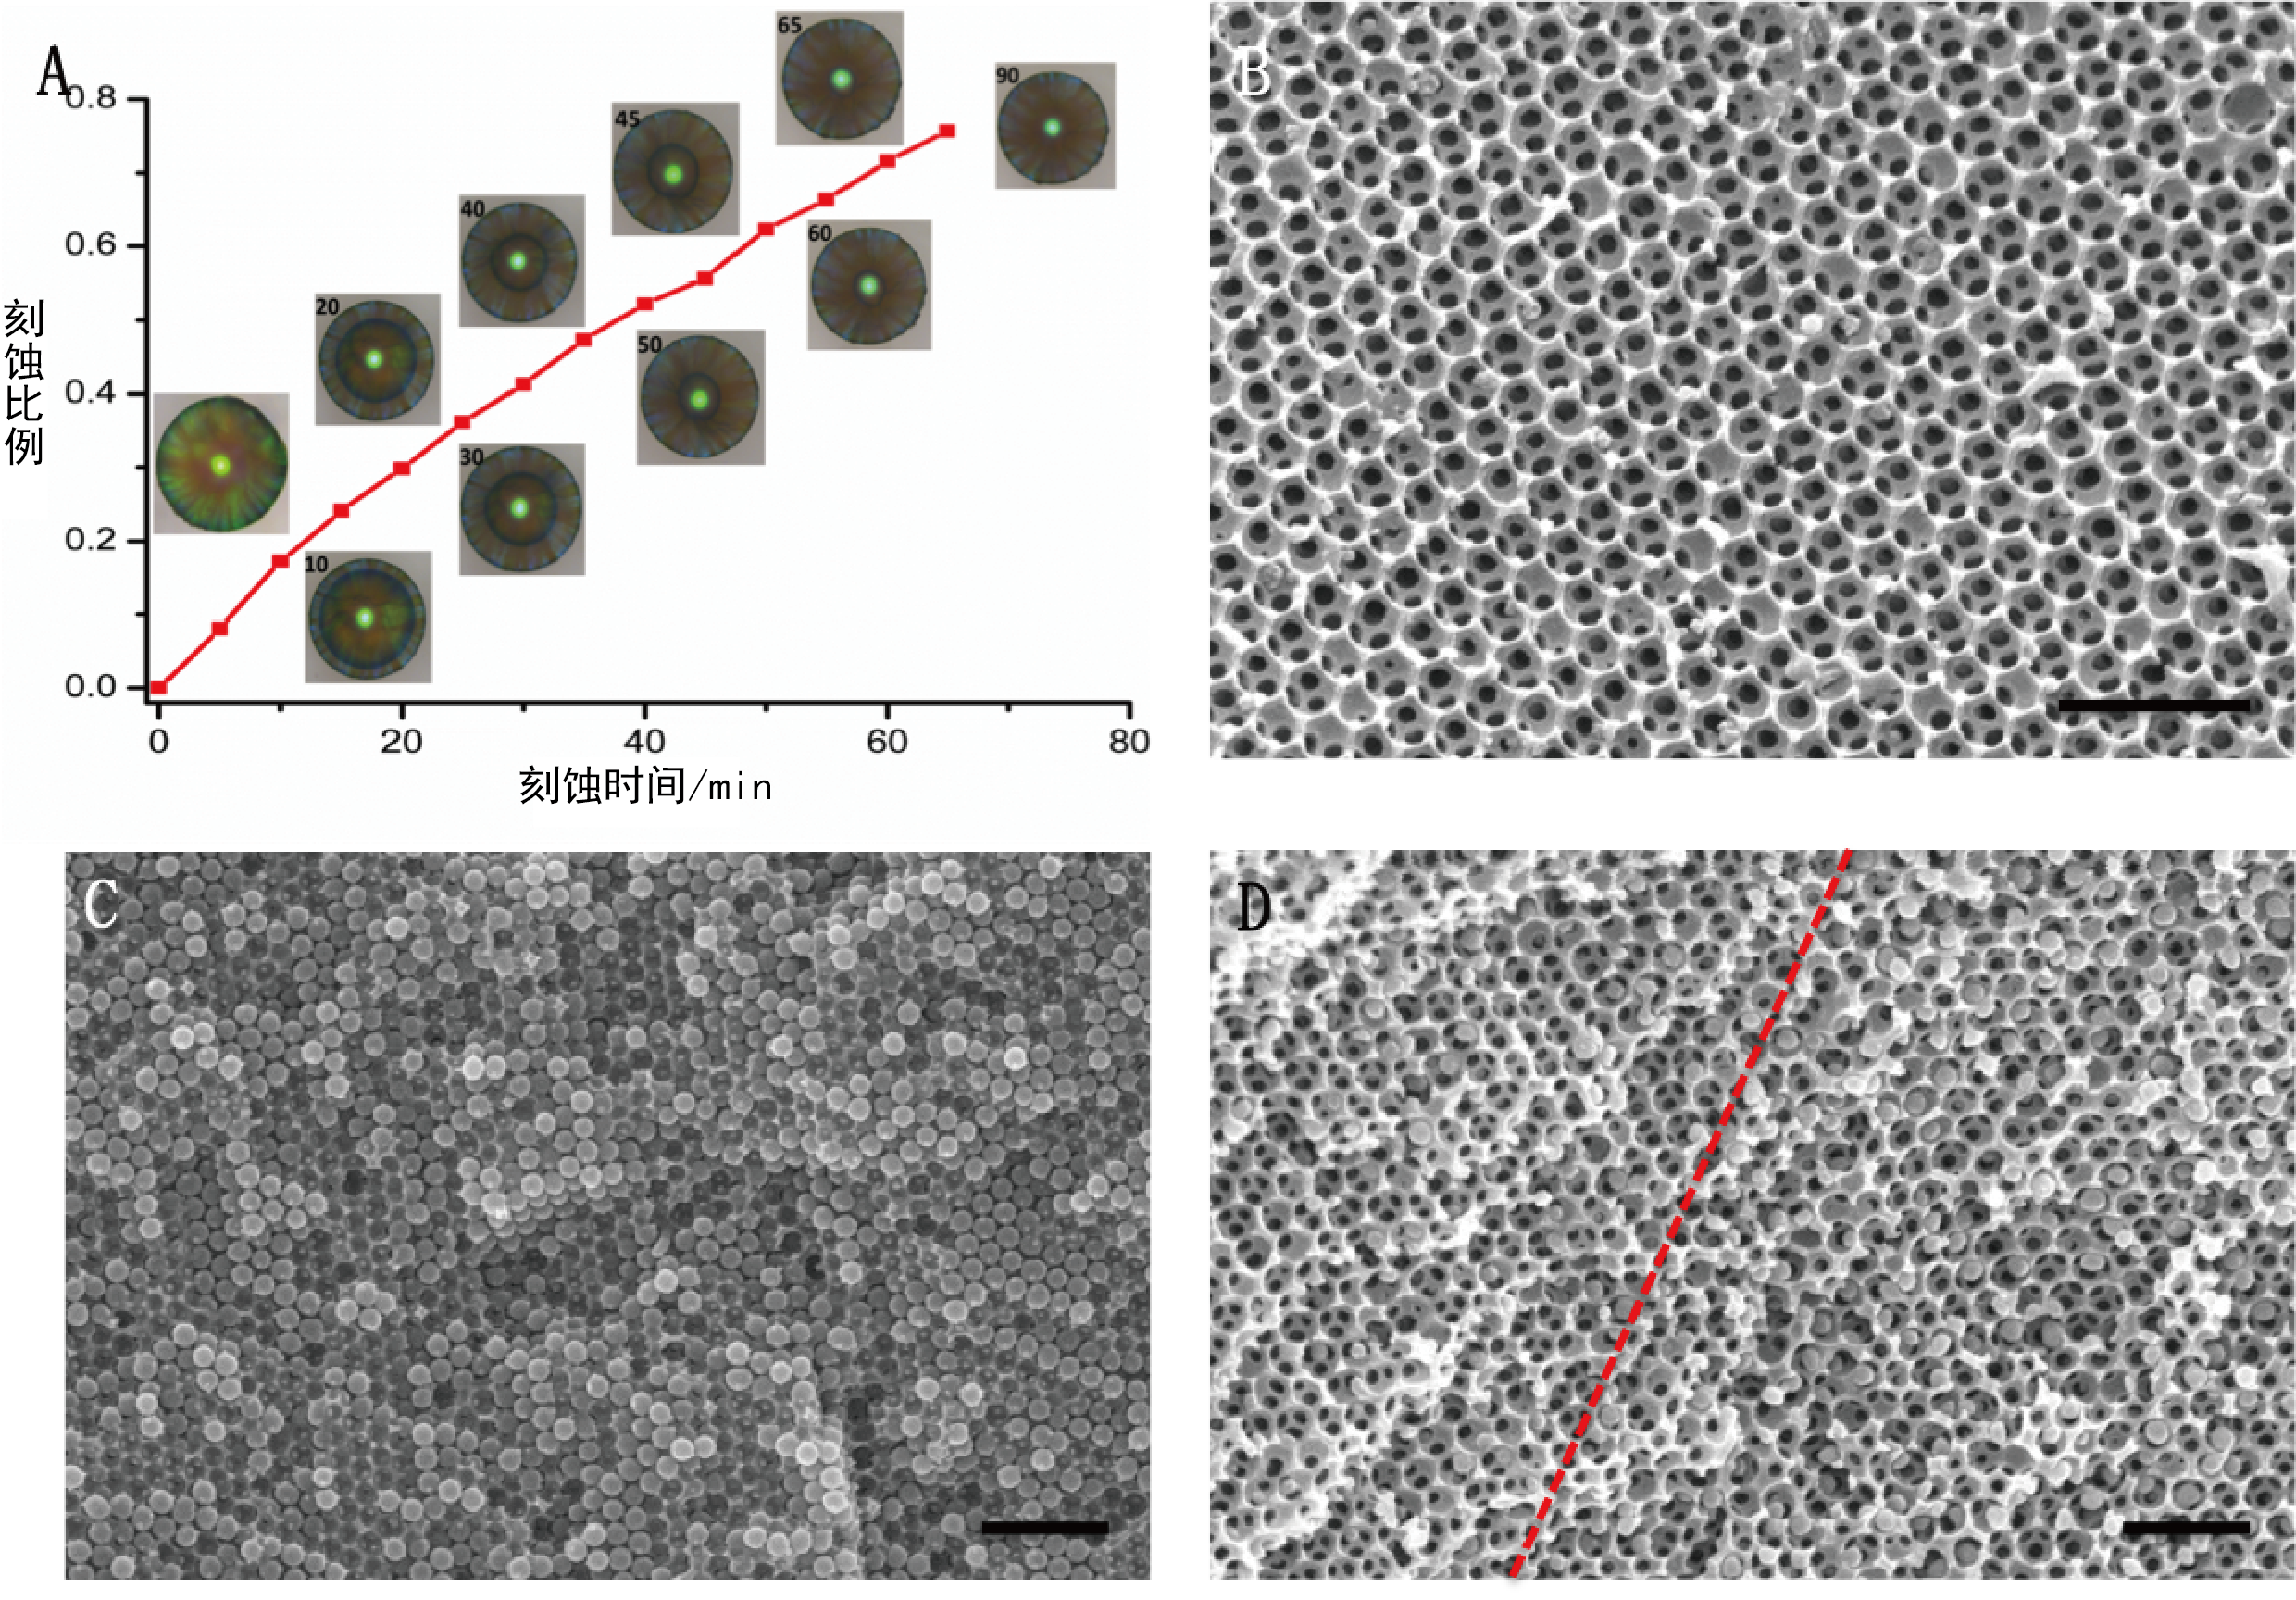
\includegraphics[width=\linewidth]{figures/ch5/Etching-exp.png}
  \caption{光子晶体微球在HF刻蚀作用下形成的结构表征。A. 光子晶体微球刻蚀程度随时间的变化关系; B. 已刻蚀部分的SEM照片;C. 未刻蚀部分的SEM照片;D. 刻蚀边界上的SEM照片。比例尺均为1 µm。}
  \label{fig:etch-exp}
\end{figure}

同时,SEM表征也显示了刻蚀边界线内外不同的结构。其中,刻蚀边界外呈现出很好的反蛋白石结构(图~\ref{fig:etch-exp}B),而在未刻蚀的内部则保持了SiO\text{$_2$}胶体颗粒的复合模板结构(图~\ref{fig:etch-exp}C)。
在两者的边界上(即显微镜中观察到的刻蚀边界)则能够观察到SiO\text{$_2$}颗粒的粒径与数目减少的趋势(图~\ref{fig:etch-exp}D)。图中的红色虚线分隔的左右两部分即呈现出不同的SiO\text{$_2$}含量,分别对应刻蚀部分与未刻蚀部分。由于中心过渡带的宽度在若干微米以下,可以认为在HF扩散刻蚀处理后的光子晶体微球被分为刻蚀与未刻蚀两部分。

\begin{figure}[htbp]
  \centering
  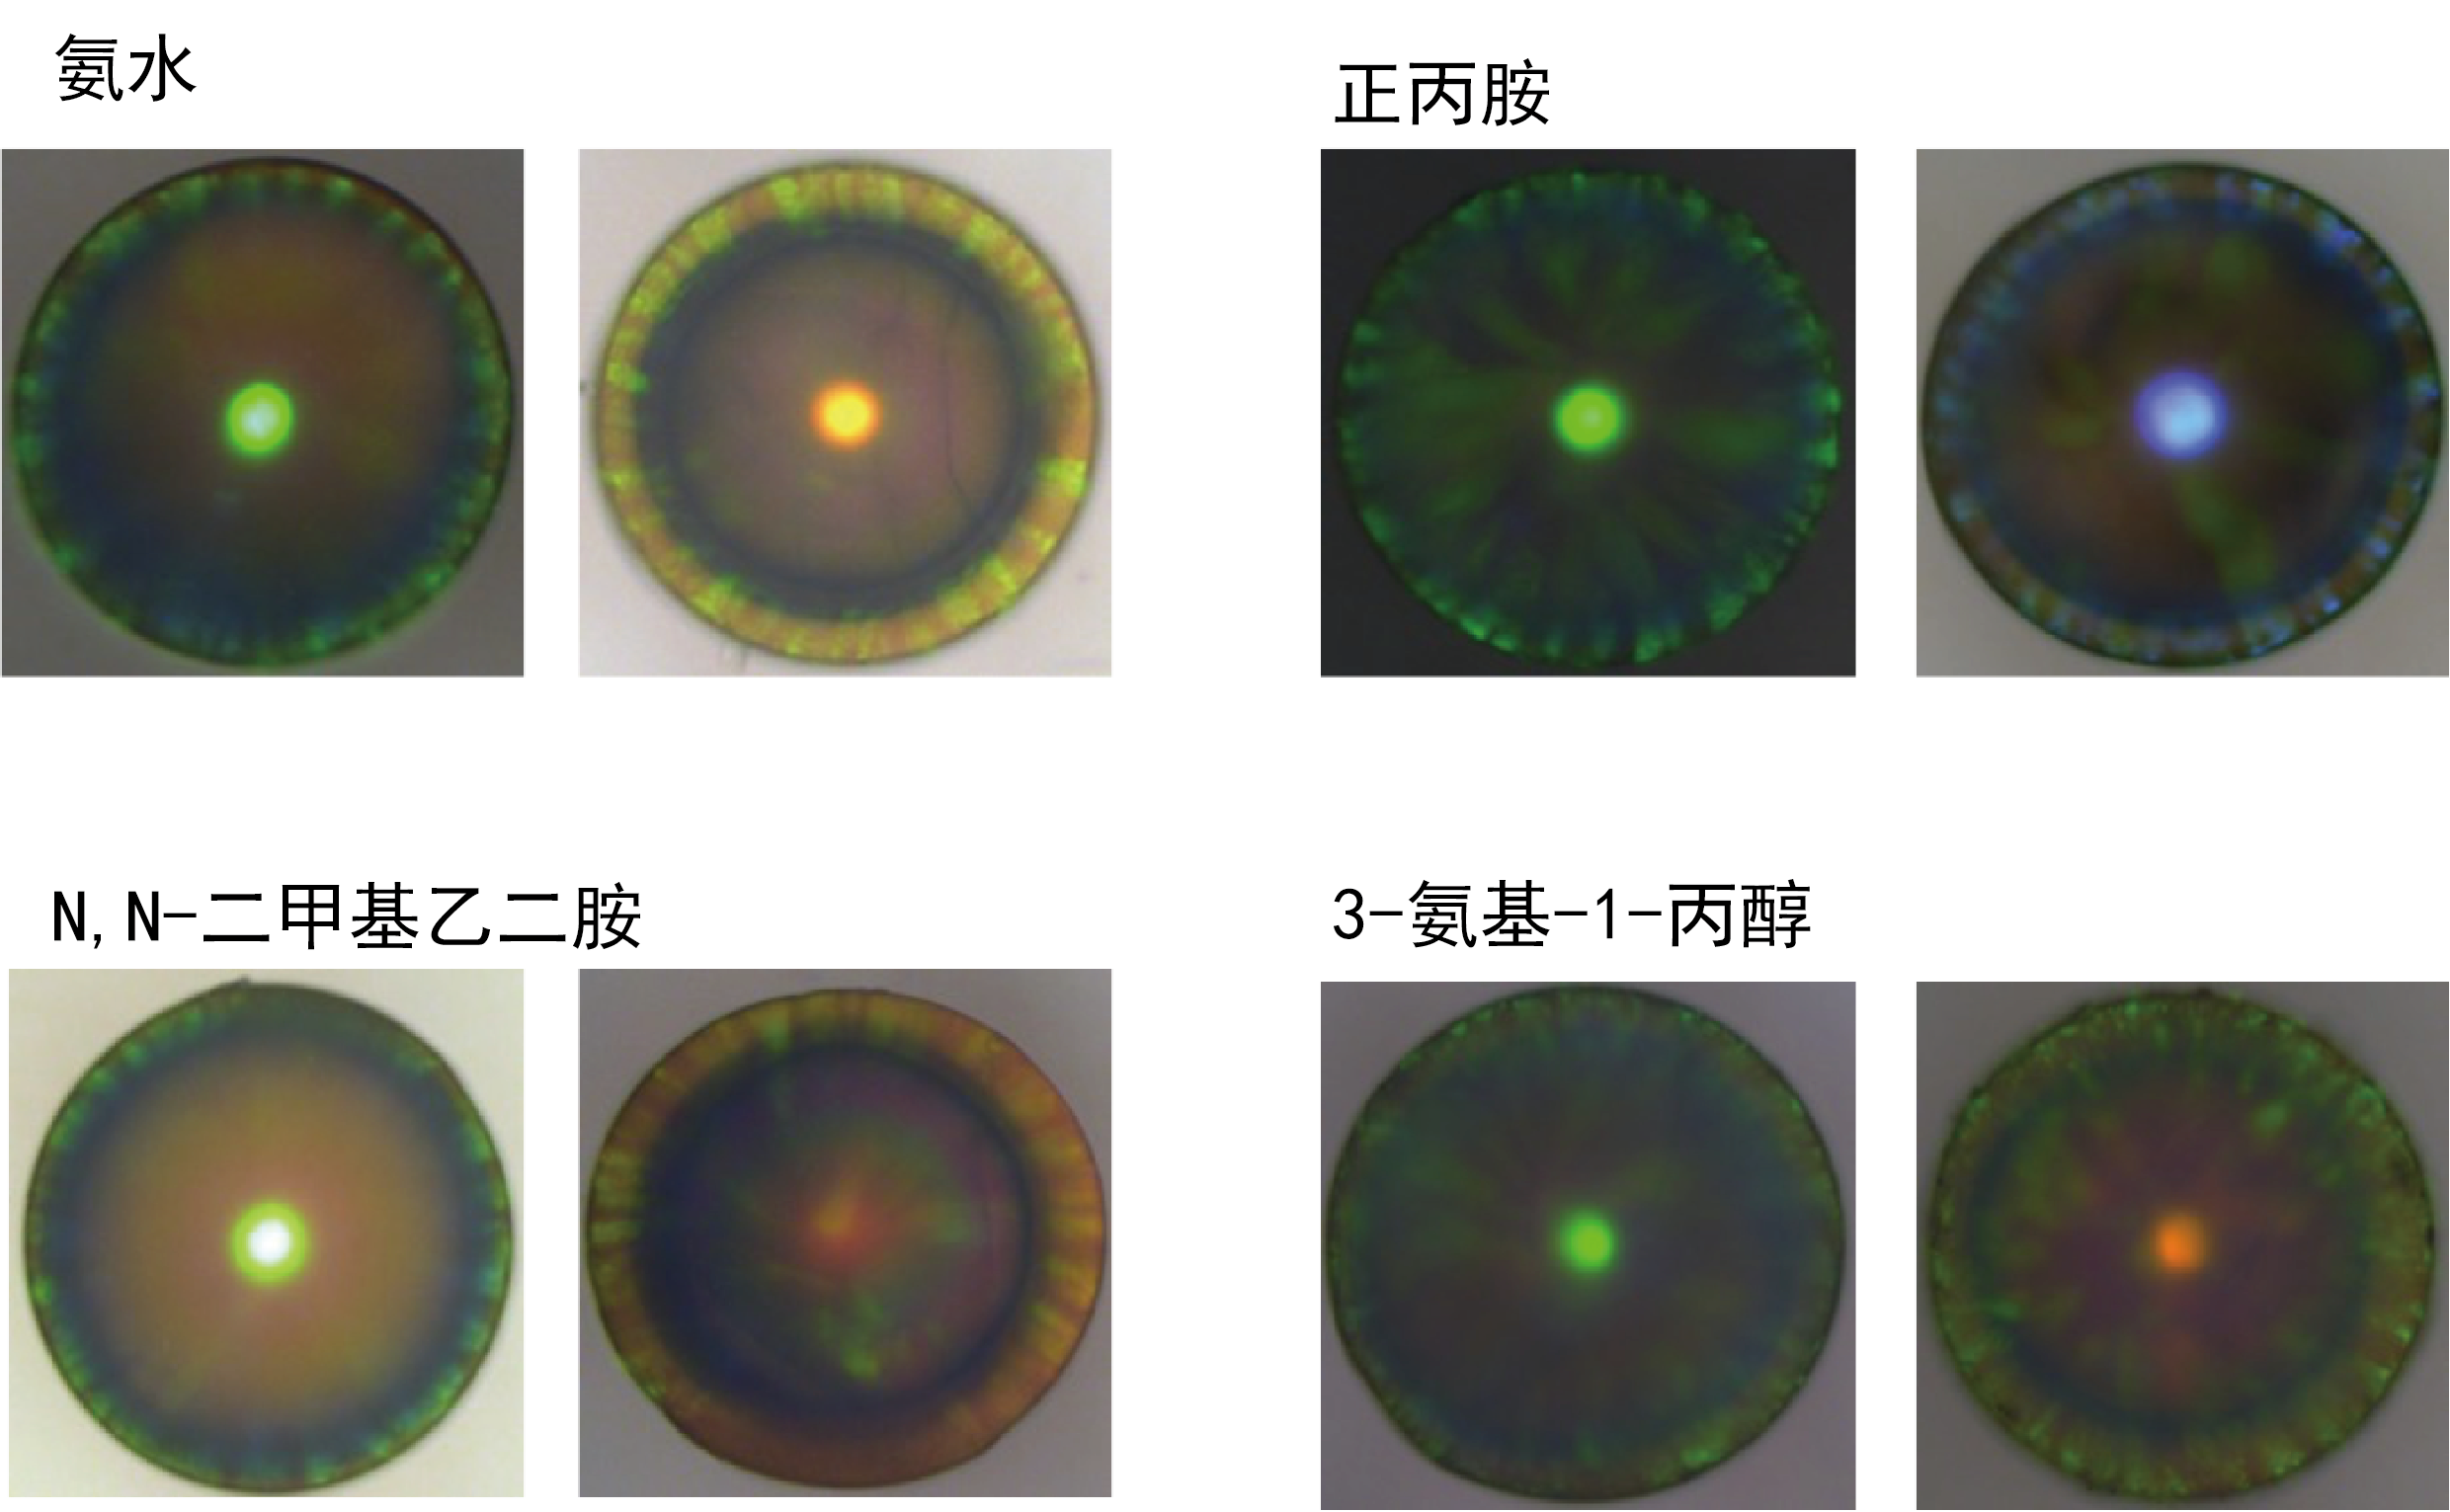
\includegraphics[width=\linewidth]{figures/ch5/etch-reaction-1.png}
  \caption{刻蚀过的光子晶体微球在不同的胺修饰前后的差异}
  \label{fig:etch-reaction-1}
\end{figure}

同时,我们也表征了修饰后的光子晶体微球的化学成分变化。如图~\ref{fig:etch-reaction-1}所示,经过不同的氨基化合物处理的光子晶体微球外层呈现不同的结构色,而内部的复合结构的结构色则几乎没有变化。同时,不同亲疏水性的胺与光子晶体反应后的结构色呈现不同的变化趋势。亲水性分子造成光子晶体的禁带红移,而疏水分子造成光子晶体的禁带蓝移,这与前述章节的预期一致。
此外,我们也通过IR光谱表征了光子晶体微球内外层在化学修饰后的差别。
由于光子晶体微球内外部较难分离,这里我们使用平面型的光子晶体薄膜进行模拟。分别使用反蛋白石型光子晶体薄膜与光子晶体复合模板在0.1 mol/L 的胺溶液或HF溶液中进行处理,清洗后进行FTIR测定。

\begin{figure}[htbp]
  \centering
  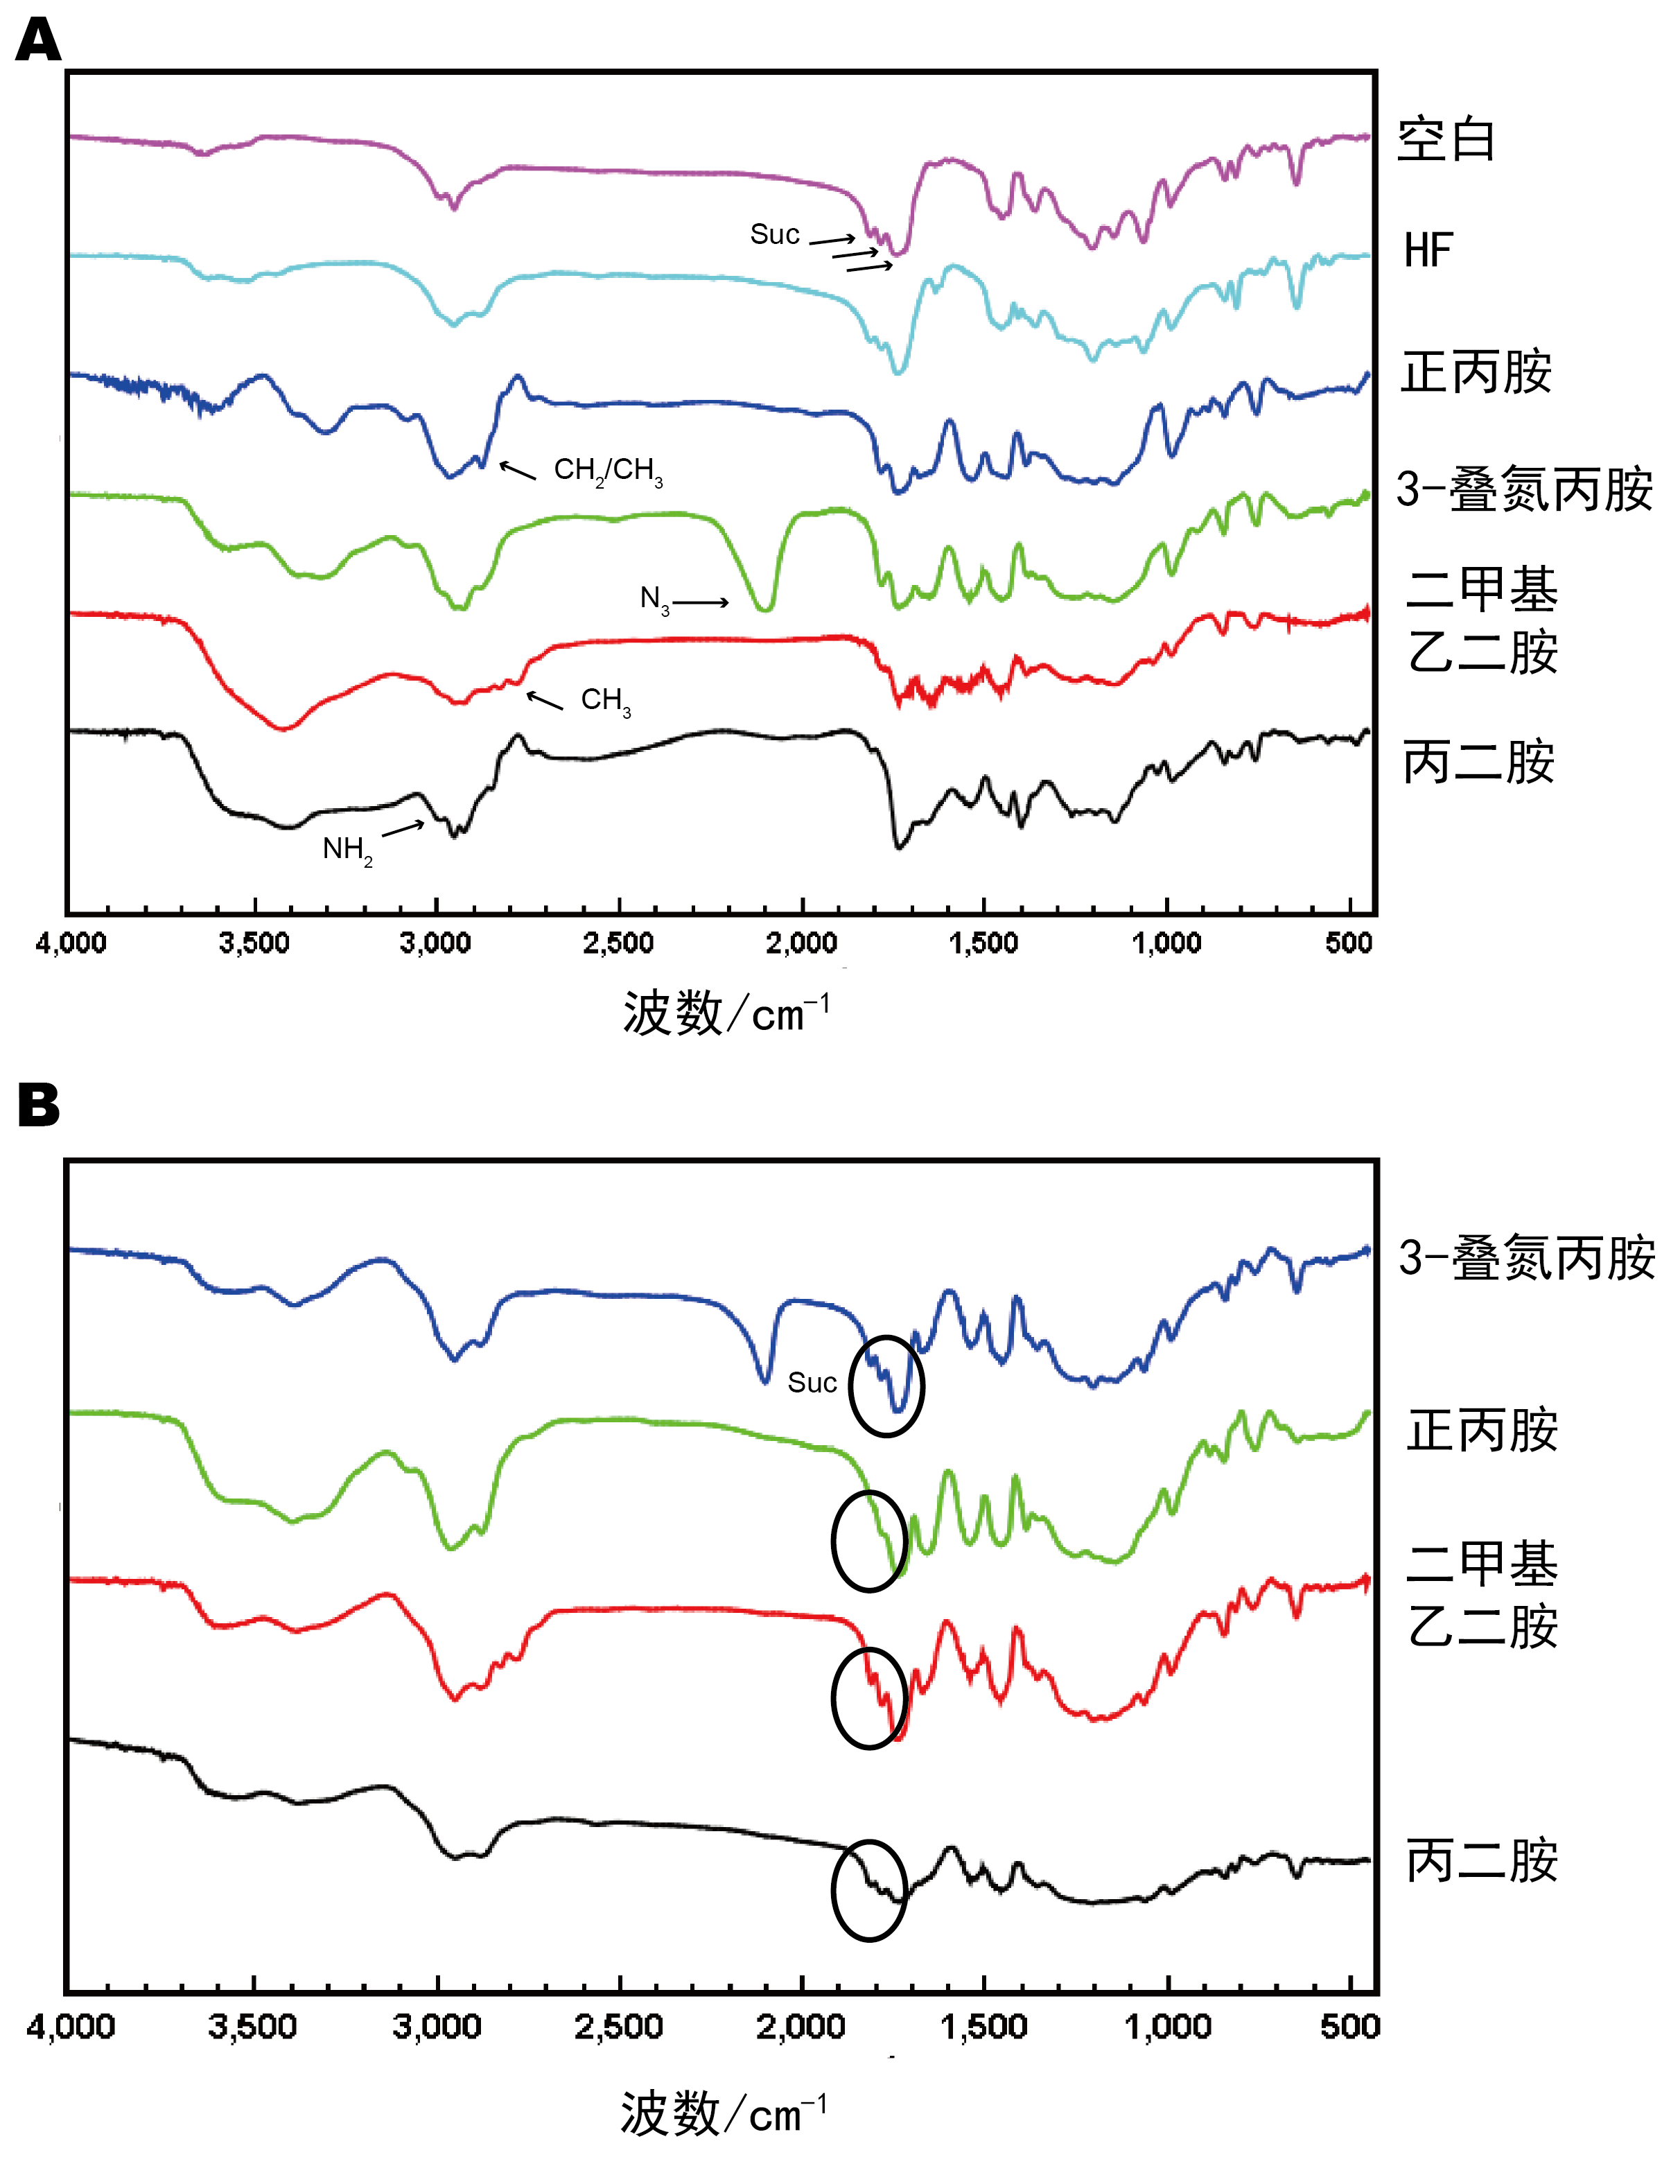
\includegraphics[width=0.85\linewidth]{figures/ch5/IR-diff.png}
  \caption{反蛋白石结构与复合结构化学修饰的差异。A. 反蛋白石结构的高分子的各种条件下修饰的IR谱图; B. 复合结构的高分子在相同条件下的修饰IR谱图。}
  \label{fig:IR-diff}
\end{figure}

如图~\ref{fig:IR-diff}A所示,含Suc活化羧基的聚合物薄膜存在1690、1780及1820 cm\text{$^{-1}$}的特征吸收峰,分别对应丁二酰亚胺的羰基及N-O振动吸收峰\cite{Guerrouache2012SiteSpecific}。
实验结果表明,HF溶液处理对聚合物中的Suc基团几乎没有影响,证明了材料在HF条件下的稳定性。
在与相应的胺反应后,可以观察到反蛋白石薄膜与复合薄膜之间的差别。反蛋白石结构的薄膜中Suc对应的特征吸收峰几乎完全消失(图~\ref{fig:IR-diff}),而在复合模板中Suc的特征吸收峰仍存在(图~\ref{fig:IR-diff}B)。此外,反蛋白石薄膜上修饰基团的对应吸收峰强度也高于复合模板中的吸收峰强度。
综合上述结果可见,反蛋白石结构的聚合物与胺的反应是完全的;而同样情况下,复合结构的光子晶体薄膜并不能实现完全的化学修饰。
这说明了反蛋白石结构的联通孔道结构能够促进物质在内部的传输,并且由孔道结构带来的巨大比表面积提升了反应的效率。相反,复合模板由于孔洞为SiO\text{$_2$}所阻塞,反应物无法进入内部,只能在表面发生反应。考虑到这里所选用的平面型光子晶体薄膜厚度(< 5 µm)与光子晶体微球内部结构的厚度相比微不足道,可以认为未刻蚀的部分几乎不受化学修饰的影响。因此,通过刻蚀-反应的方法能够实现光子晶体微球中的差异性化学修饰需求。

除了表征通过刻蚀-反应方法实现光子晶体微球中差异的化学成分以外,我们还对这种方法制备光子晶体微球多层结构的精确性进行了研究。
这里我们采用合成的氨乙基罗丹明B(化合物11)作为标记物对光子晶体微球进行标记。这里我们分别进行两方面的表征,分别为所制备的层状结构的厚度与其位置。

\begin{figure}[htbp]
  \centering
  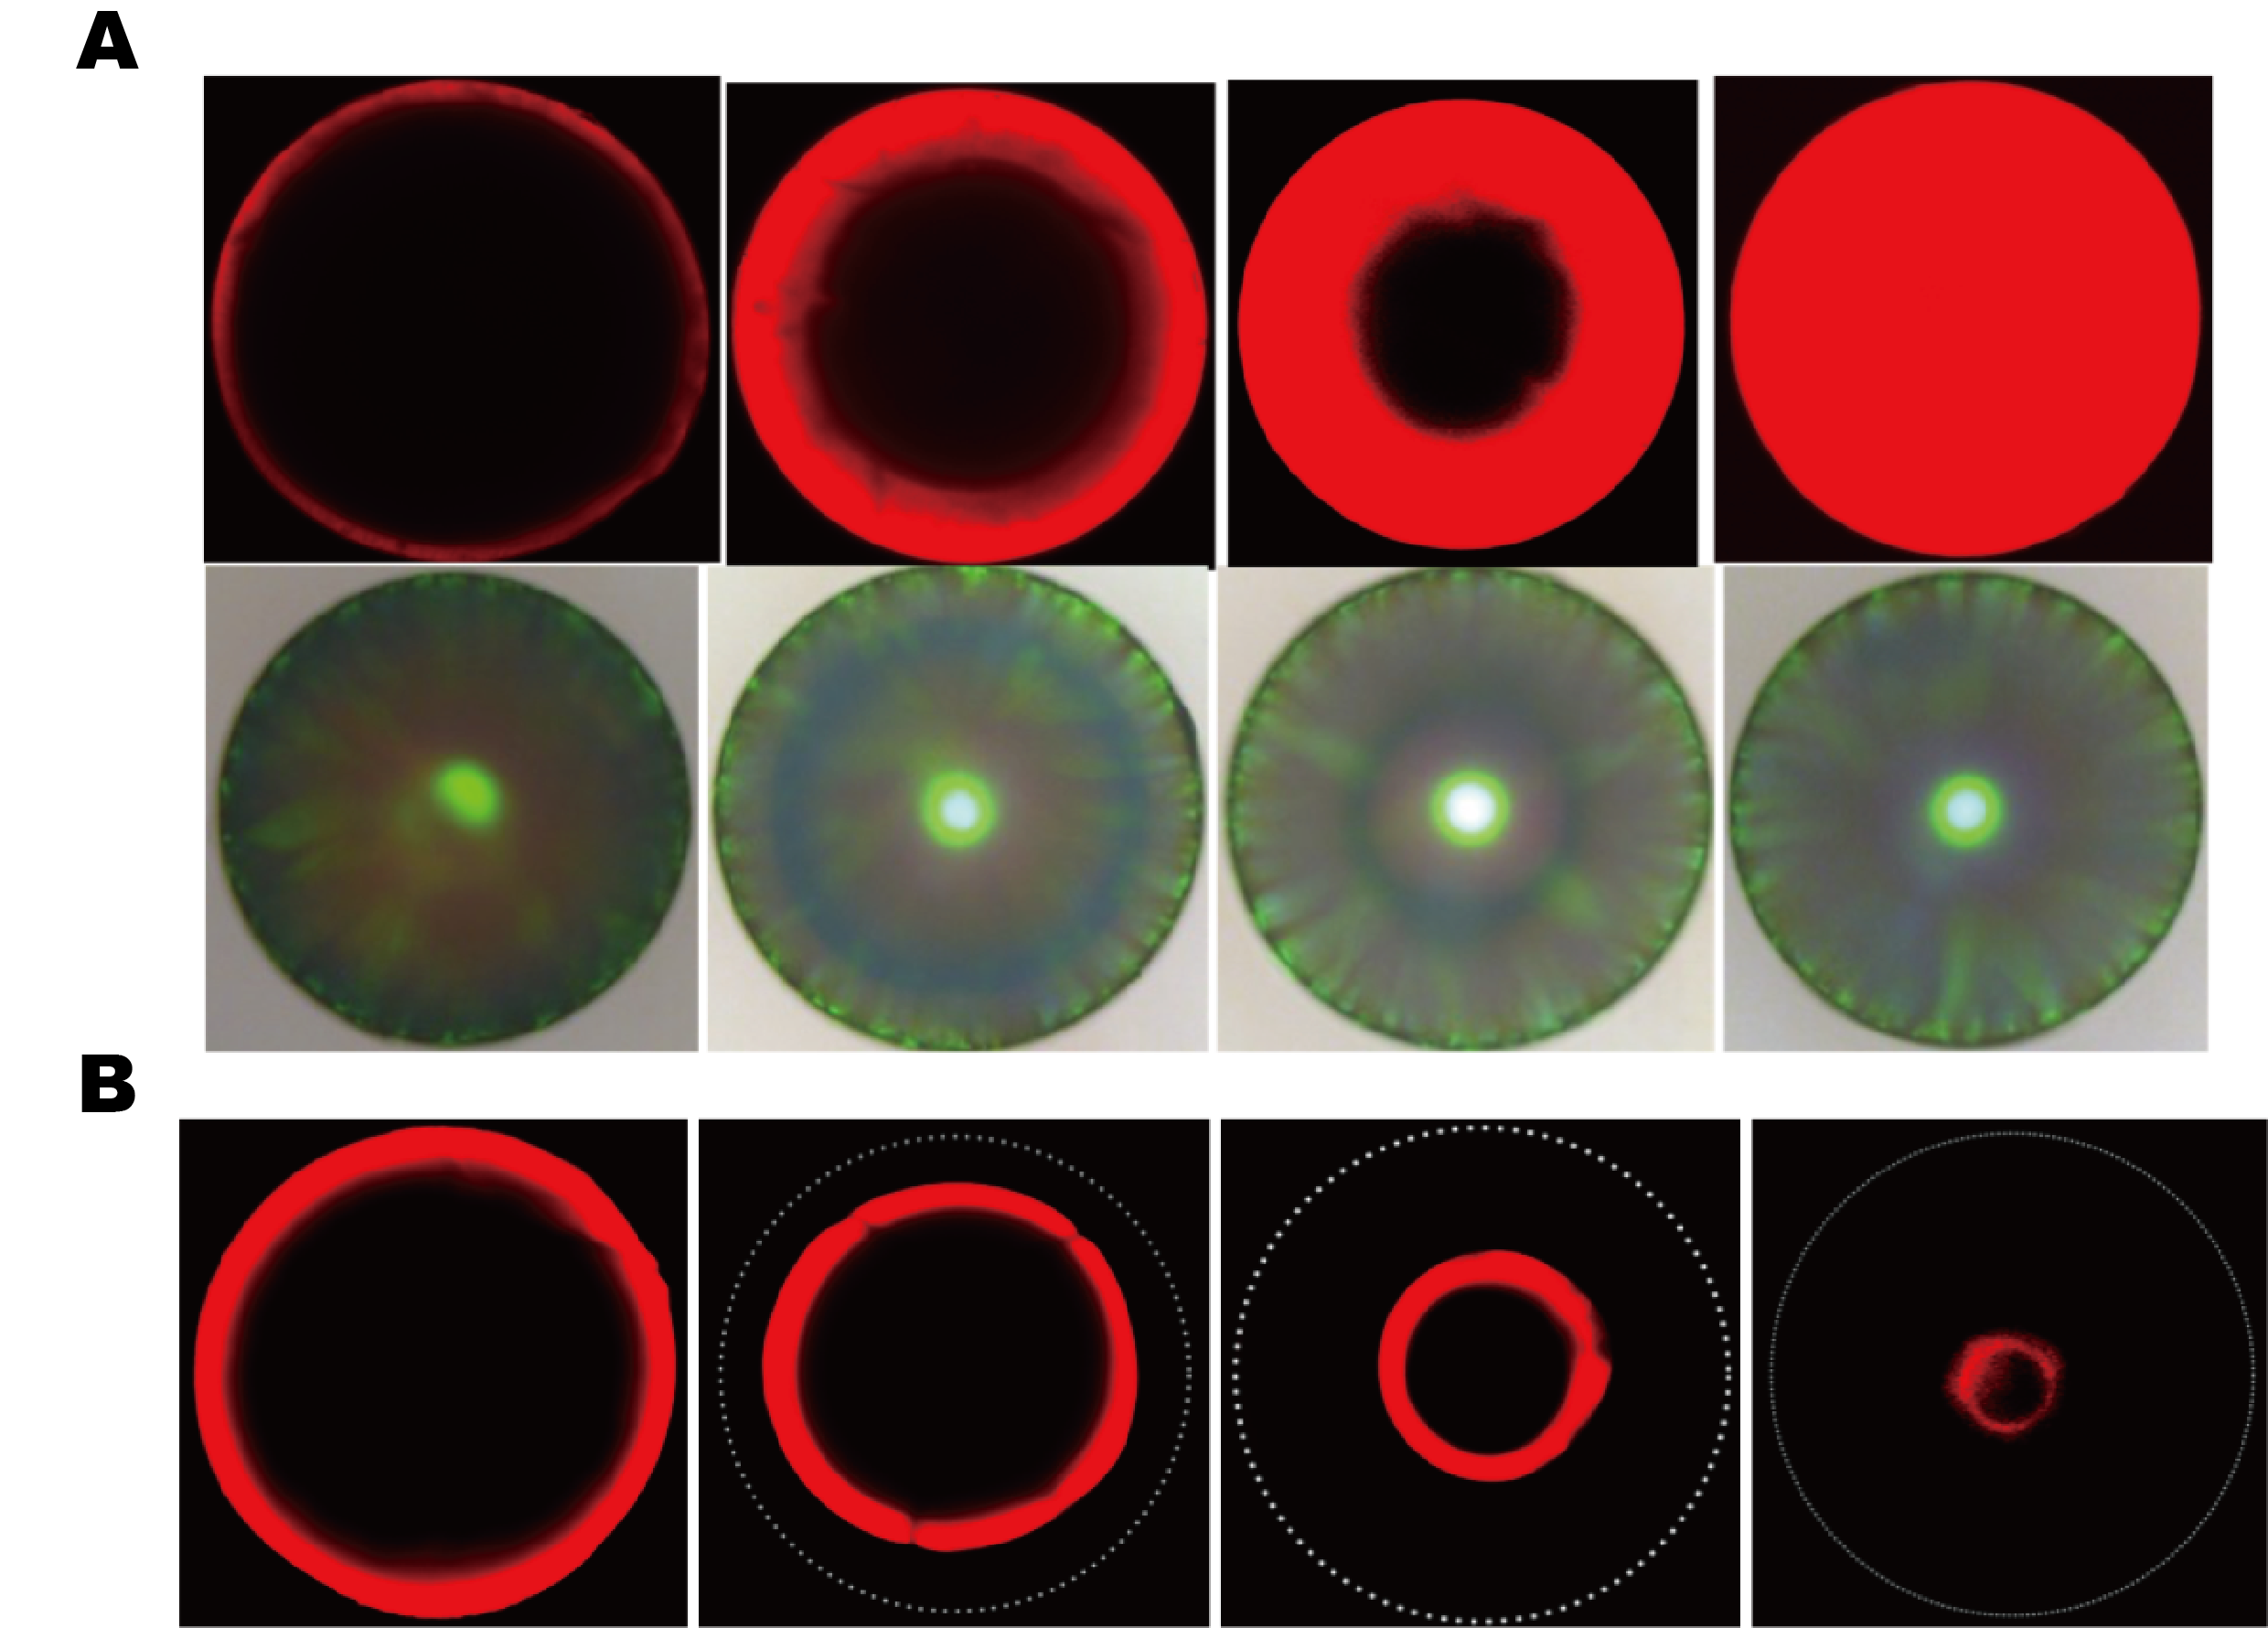
\includegraphics[width=\linewidth]{figures/ch5/RhB-dye.png}
  \caption{刻蚀-反应法对光子晶体微球多层结构的调控,并通过化合物11标记物进行CLSM及光镜的表征照片。A. 对外层厚度的调控;B. 对内层位置的调控 }
  \label{fig:RhB-dye}
\end{figure}

如图~\ref{fig:RhB-dye}A所示,对最外层的荧光染色结果显示荧光标记物均匀分散在外层中,且外层的相对厚度可从小于10 \%逐渐增加到100 \%,与光学照片相对应,说明这种化学修饰方式在反蛋白石结构中是均匀发生的。
更为重要的是,由于Suc活化羧基与氨基化合物反应的充分性,可以做到目标化合物的空间选择性修饰。如图~\ref{fig:RhB-dye}B所示,染色的内层结构与中心的距离可以进行调控且
在内层被荧光标记物染色的同时,外层的反蛋白石结构没有显示荧光信号,说明通过各层的完全修饰可以实现目标化合物的精确、无交叉定位反应。

上述实验结果证明了这种利用刻蚀-反应的修饰方法能够实现在光子晶体微球中的差异性修饰。同时,结合了刻蚀过程的可控性与修饰反应的充分性,能够实现对光子晶体微球多层结构的层数、位置、厚度、组分的调控。这种多层光子晶体微球能够作为一种高度可拓展的平台,并可在此基础上发展一系列功能材料。

\subsection{具有三维亲疏水梯度的光子晶体微球材料及其表征}

受上一节中利用Suc活化羧基与不同胺类化合物反应带来的亲疏水性差异的启发,我们希望结合多层的化学修饰法在光子晶体微球内部构造三维尺度上的亲疏水结构。
这里我们分别使用了DMEA、AP、DDA三种由亲水到疏水的胺类化合物对光子晶体微球进行化学修饰。
首先我们利用接触角表征了不同的胺与活化羧基聚合物反应后的亲疏水性。
\begin{figure}[htbp]
  \centering
  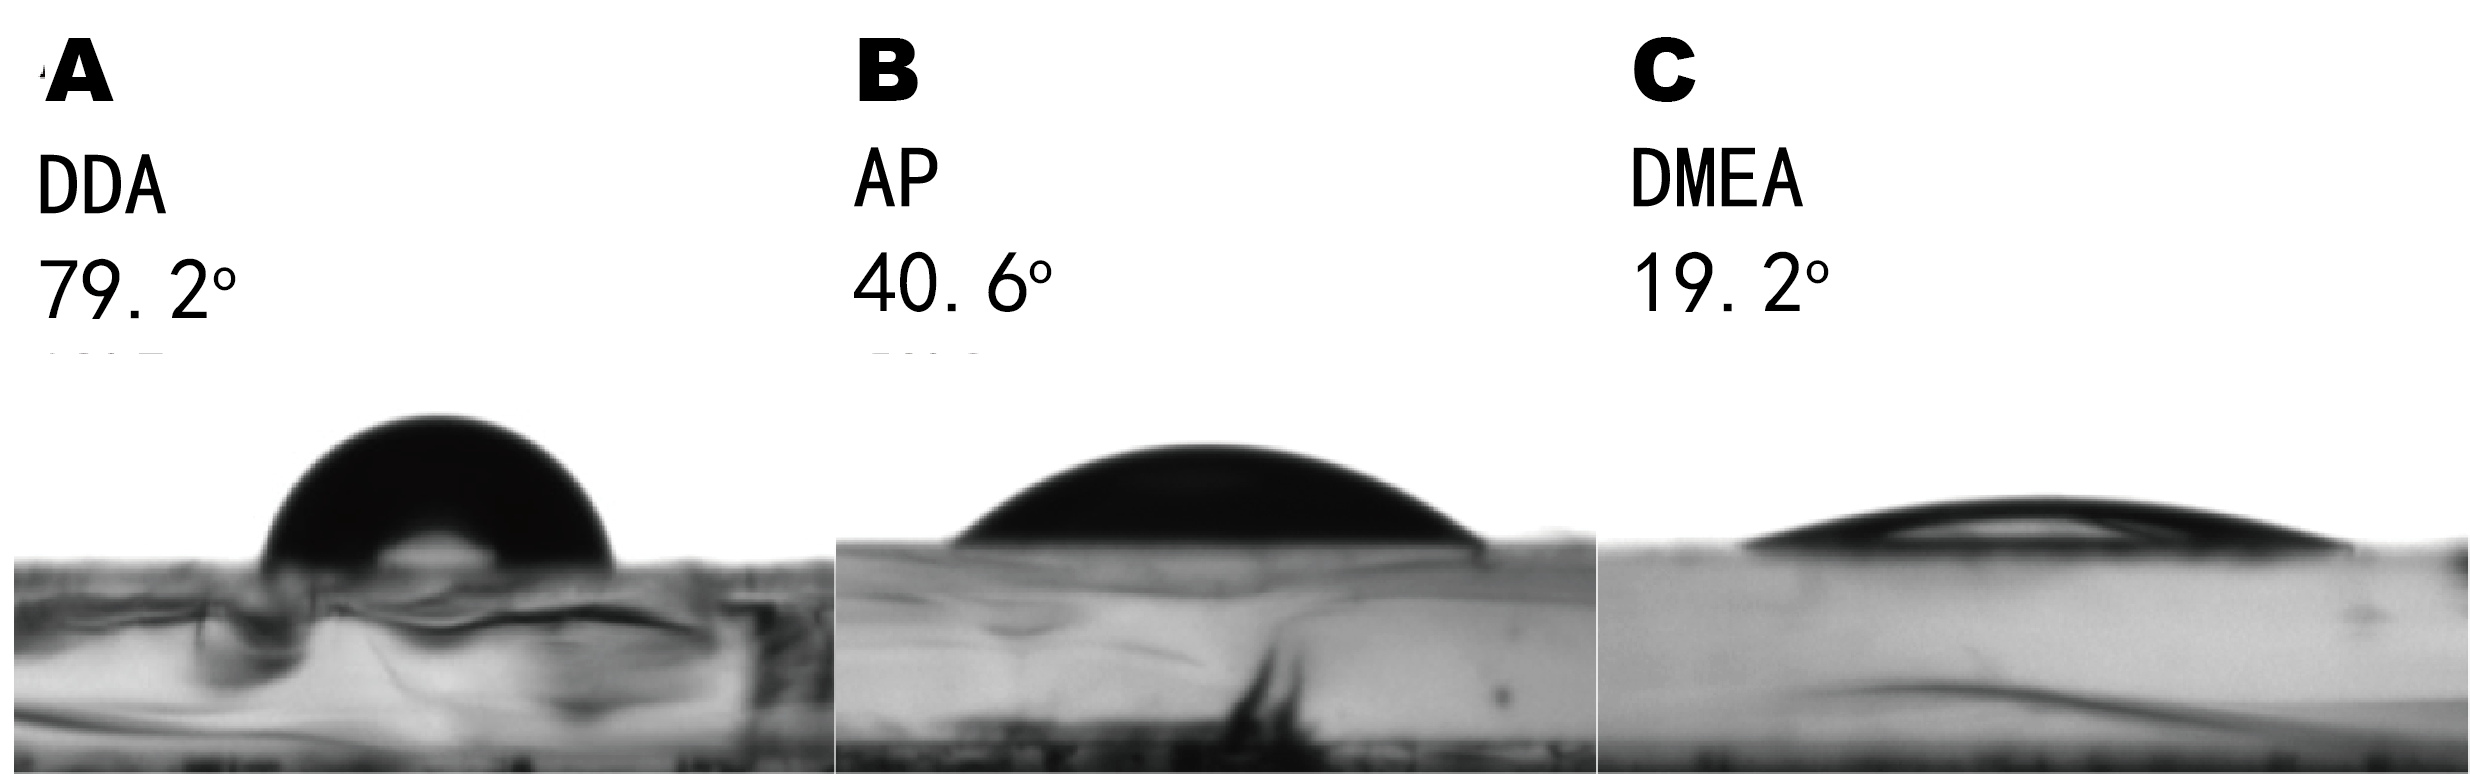
\includegraphics[width=\linewidth]{figures/ch5/ch5-CA.png}
  \caption{Suc活化羧基高分子在不同的胺修饰后的接触角差异}
  \label{fig:ch5-CA}
\end{figure}

如图~\ref{fig:ch5-CA}所示,
DDA修饰后的聚合物的接触角为79.2$^\circ$。其较为疏水的特性来自于DDA中长链烷基链。而AP修饰的聚合物的接触角为40.6$^\circ$,其亲水性与末端的羟基基团有关。而DMEA修饰的聚合物的接触角则更小,达到了19.2$^\circ$。这些接触角结果与预期一致。
三者的亲疏水性的连续变化使其能够用来构筑光子晶体微球中三维尺度上的亲疏水性梯度。

如图~\ref{fig:CCB-gradient}A所示,利用刻蚀-反应法制备的具有亲疏水梯度的光子晶体微球由三层组成,从外到内分别修饰了DMEA、AP以及DDA。
\begin{figure}[htbp]
  \centering
  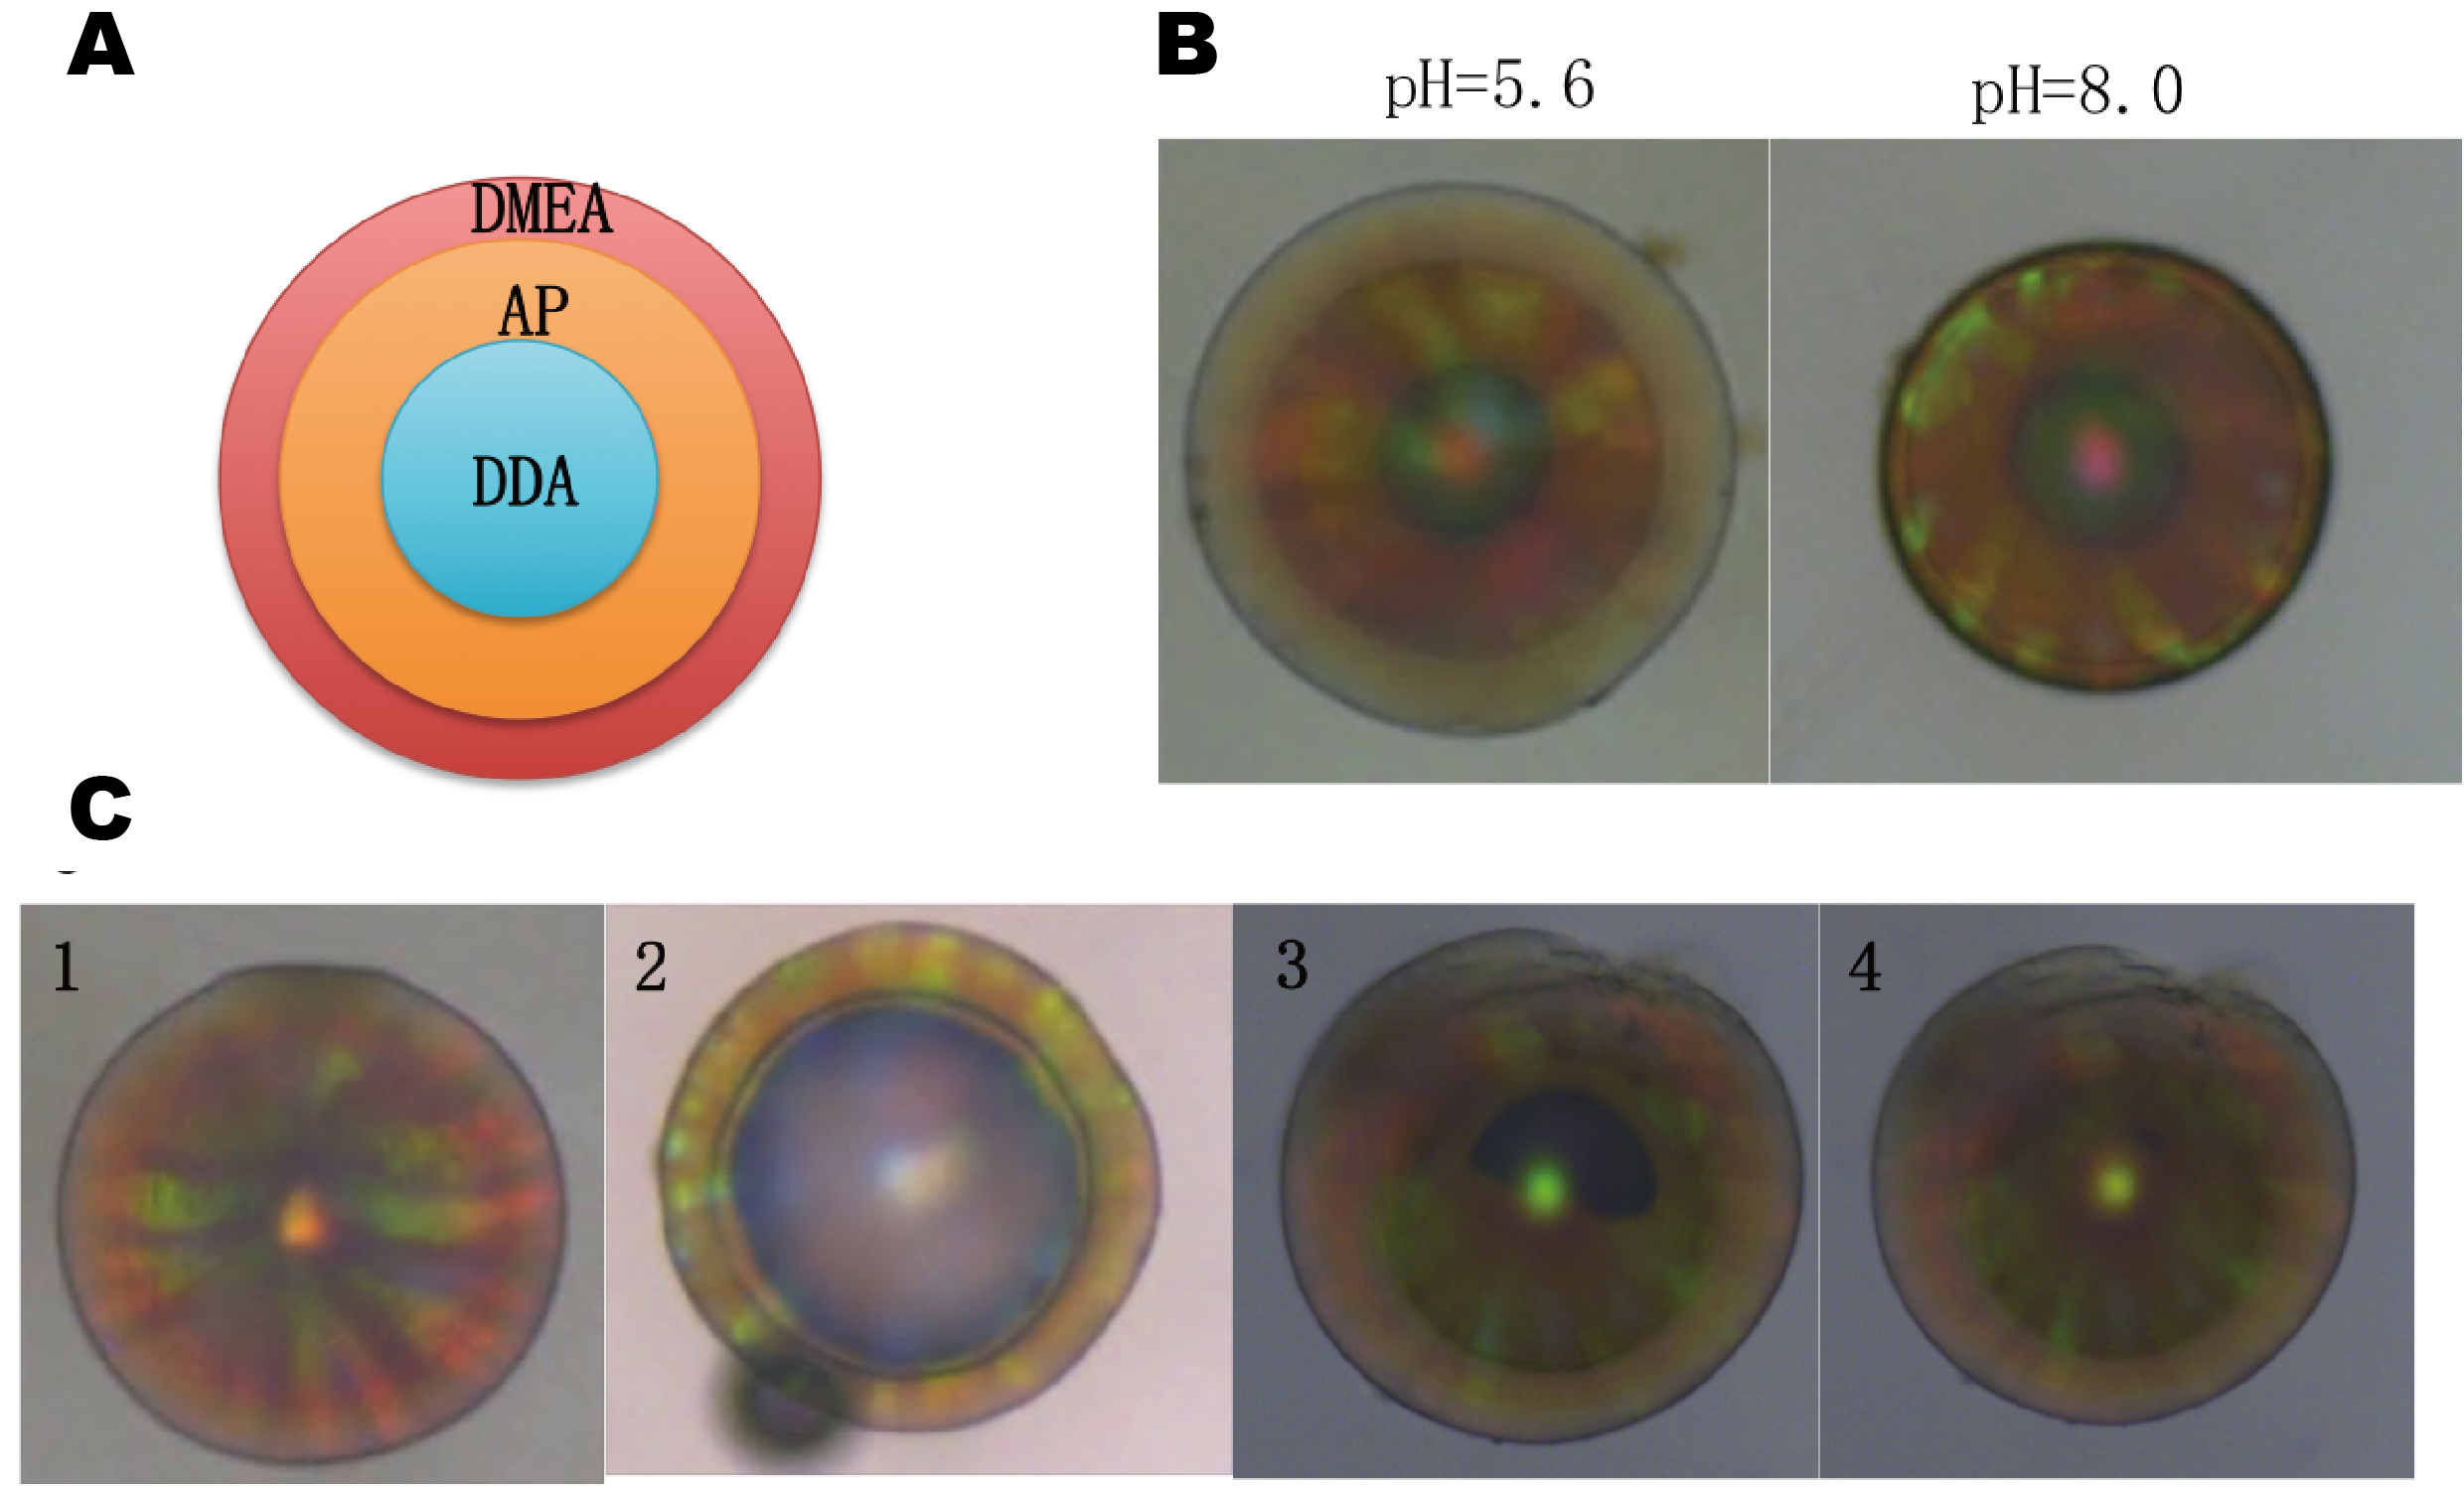
\includegraphics[width=\linewidth]{figures/ch5/CCB-gradient.png}
  \caption{刻蚀-反应法在光子晶体微球中实现亲疏水梯度结构。A. 光子晶体微球各层示意图;B. 亲疏水梯度的光子晶体微球的pH响应门控效应;C. 亲疏水梯度带来的有机溶剂选择性通透效应}
  \label{fig:CCB-gradient}
\end{figure}
这种亲疏水梯度特性能够在光子晶体结构色上体现出来。可以在观察到图~\ref{fig:CCB-gradient}B中三层结构的结构色从外至内呈现蓝移的趋势,对应其疏水性的增加。此外,由于DMEA的三级胺头基结构,使得其在不同pH下的质子化状态存在差异。在pH=5.6时,外层的DMEA被质子化,使得最外层呈现较大的禁带红移及体积;而在pH=8.0的碱性条件下是,DMEA去质子化而亲水性降低,最外层的光子晶体结构发生收缩。
由于所处环境为较为温和的pH值,这种质子化-去质子化的过程具有可逆性\cite{Siegel1988PhDependent}。同时,内部的光子晶体结构则不受pH变化影响。因此,外层的反蛋白石结构构成了一个pH可控的动态通透性壳。pH动态调节的特性使其在对胶体颗粒的动态门控等方面具有潜在的应用\cite{Yang2013MaleimideContaining}。

更为有趣的是,这种连续的亲疏水梯度能够带来定向的液体通透调控(图~\ref{fig:CCB-gradient}C)。为了便于观察,这里我们制备了同样具有DMEA-AP-DDA三级亲疏水梯度结构的光子晶体微球,但前两层结构的厚度远小于第三层。也即光子晶体微球内部主要为疏水的核心,由逐渐亲水的外层壳包裹。在光子晶体逐层修饰的过程中,由于使用了乙醇等有机溶剂浸润,使得光子晶体微球内部孔道均为水填充,呈现相同的衍射特性。
但将光子晶体微球内部的水干燥去除后,这种具有亲疏水梯度的光子晶体微球在重新水化的过程中呈现出不同的浸润性:外层的DMEA/AP修饰层能够恢复原始的结构色,说明水进入了这两层反蛋白石的孔道内;而疏水的最内层则呈现灰白的各向同性外观。结构色的消失说明水没有渗透入最内层反蛋白石的孔道中,而内层为空气所填充。
这种在水化过程中浸润性的差异是由亲疏水性差异与反蛋白石孔道的结构共同决定的\cite{Burgess2012Wetting}。
同时,我们发现当在水中加入少量的有机溶剂(例如甲苯)之后,内部的空气屏蔽的反蛋白石孔道会逐渐被再次浸润。这是由于甲苯对于亲水性或疏水性的部分均具有较小的接触角,使得内部孔道能够对其通透。同时,在甲苯溶剂向内渗透的同时,也将水带入最内层的孔道中,从而将内部孔道浸润。
上述性质说明亲疏水性梯度与光子晶体孔道的结合能够形成对水-有机溶剂选择性通透
的功能体系。外层到内层逐渐疏水的梯度作为一种“驱动力”使得其对有机溶剂具有定向通透性。这种功能体系能够作为良好的有机溶剂富集材料,并能够通过光子禁带的变化直观地反映亲疏水性的变化,在油水分离等实际应用中具有潜在应用。

\subsection{具有正交化学活性的光子晶体微球材料及其表征}

除了基于Suc活化羧基-氨基的反应进行光子晶体修饰,使其获得静态的化学成分以外,还可以利用这种反应-修饰方法使光子晶体获得二次反应活性,使一些原本难以用于制备聚合物单体的活性基团能够被修饰到光子晶体上。
这里,我们选择在光子晶体微球中接枝具有正交化学活性的官能团,以实现对光子晶体的二次修饰。
正交化学反应是一系列条件温和、反应高效的反应,且其最大特征是正交化学组合之间不会发生交叉反应。正交化学的活性与选择性使其在生物接枝、超分子修饰等方面具有广阔的应用\cite{Agard2006Comparative,Elacqua2014Engineering}。正交化学反应使得在化学修饰在空间上具有特异性,而结合这里的刻蚀-反应修饰法,我们希望能够在光子晶体微球内部形成具有空间层次的正交化学反应活性。

这里我们采用了三组正交化学反应组合,分别为叠氮-活化炔基、氨基-异硫氰酯、Suc活化羧基-氨基
其中由于光子晶体微球自身的组成原因,Suc活化羧基为最内层,其余两层分别接枝修饰叠氮与氨基。
相对应的,我们分别采用了具有特异性基团的荧光标记分子来对正交化学反应进行标记。这里采用的荧光标记分子为:异硫氰荧光素(FITC)、环辛炔偶联罗丹明B(CO-RhB,化合物16),以及氨基瀑布蓝(CBa,化合物18),分别对应氨基、叠氮及Suc活化羧基。

我们首先利用原位CLMS观察了荧光标记分子在正交化学体系中的反应性,使用FITC与CO-RhB分别对含有氨基及叠氮基团的光子晶体多层结构进行荧光标记。
\begin{figure}[htbp]
  \centering
  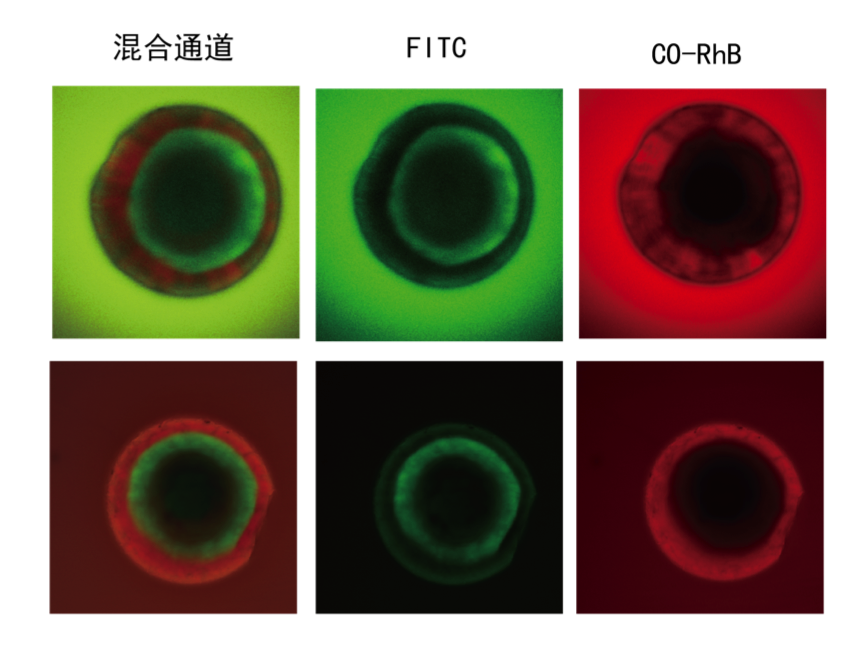
\includegraphics[width=\linewidth]{figures/ch5/livestaining.png}
  \caption{光子晶体微球中二元正交化学组合的实时平行染色实验。}
  \label{fig:livestaining}
\end{figure}
如图~\ref{fig:livestaining}所示,在原位反应的条件下,只有与标记分子对应的正交化学区域才显示出增强的荧光信号,而在其他区域则没有被荧光标记物修饰,说明了正交化学荧光标记的可行性。
在此基础上,我们分别采用三种荧光标记分子对具有正交化学活性的光子晶体微球进行荧光标记(图~\ref{fig:tristain})。
\begin{figure}[htbp]
  \centering
  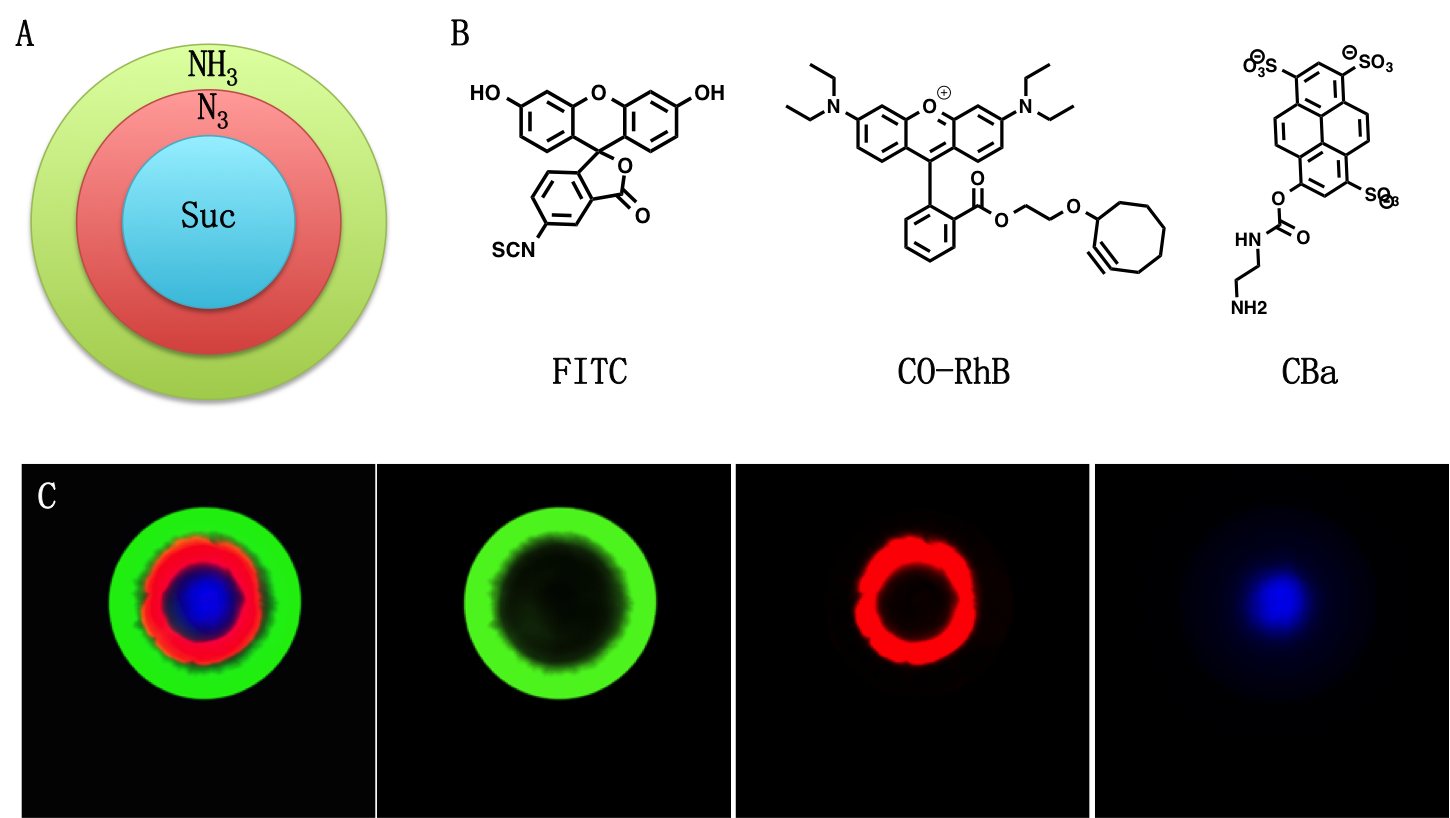
\includegraphics[width=\linewidth]{figures/ch5/Tristain.png}
  \caption{三元正交化学反应组合在光子晶体微球中的实现。A. 光子晶体微球内部的修饰化学成分示意图; B. 本节中所选用的对应的荧光标记化合物;C. 荧光标记物对光子晶体内部选择性修饰的CLMS照片}
  \label{fig:tristain}
\end{figure}

CLMS图片结果显示不同的块区之间具有高度的正交性,可以从单通道荧光照片看出区域之间几乎没有交叉沾染的现象,且荧光强度均匀,说明了所选的正交化学反应组合在光子晶体微球中能够实现化合物的平行无交叉修饰。本节中利用荧光标记染料作为示例展示了光子晶体微球中三维正交化学活性结构的可行性,这种空间上的特异性化学修饰方法与光子晶体微球特性结合,大大提高了光子晶体的拓展性。而这种正交化学体系可以进一步发展以实现其他分子乃至蛋白质的正交修饰\cite{Rahmani2014Chemically},以实现更为复杂的功能体系。

\subsection{级联反应的光子晶体微球材料及其表征}
刻蚀-反应方法制备的光子晶体微球中的多层结构之间具有空间相邻的特性,使得各层结构之间的协同与交互作用成为可能。
在此基础上,我们尝试在光子晶体微球中实现多重生物酶的修饰,并形成级联反应体系。同时,利用光子晶体信号自表达特性与化学发光法来表达这种酶的级联反应。
本节中所选用的酶的级联体系为乙酰胆碱酯酶(AChE)-胆碱氧化酶(ChOx)-辣根过氧化酶(HRP)。
其中,乙酰胆碱(ACh,或其模拟物乙酰巯基胆碱ATCh)在AChE作用下水解生成胆碱;胆碱作为ChOx的底物参与第二步反应,在有氧气存在环境下被氧化,生成氧化产物H\text{$_2$}O\text{$_2$};而H\text{$_2$}O\text{$_2$}进一步成为第三步反应中HRP的底物,被催化分解为活性氧。
而在信号表达方面我们采用了双信号表达体系。一方面,级联反应的终产物可以对一系列标记物氧化而产生信号,包括2,2'-联氮双(3-乙基苯并噻唑啉-6-磺酸)二铵盐(ABTS)以及卢米诺等;同时,若反应起始底物使用ATCh,第一步的反应产物TCh可以利用第~\ref{ch:maleimide}中的马来酰亚胺基团进行捕捉并产生光子晶体禁带偏移。这种具有双信号表达的级联反应光子晶体微球的原理可见于\
图~\ref{fig:cascade-principle}。
\begin{figure}[htbp]
  \centering
  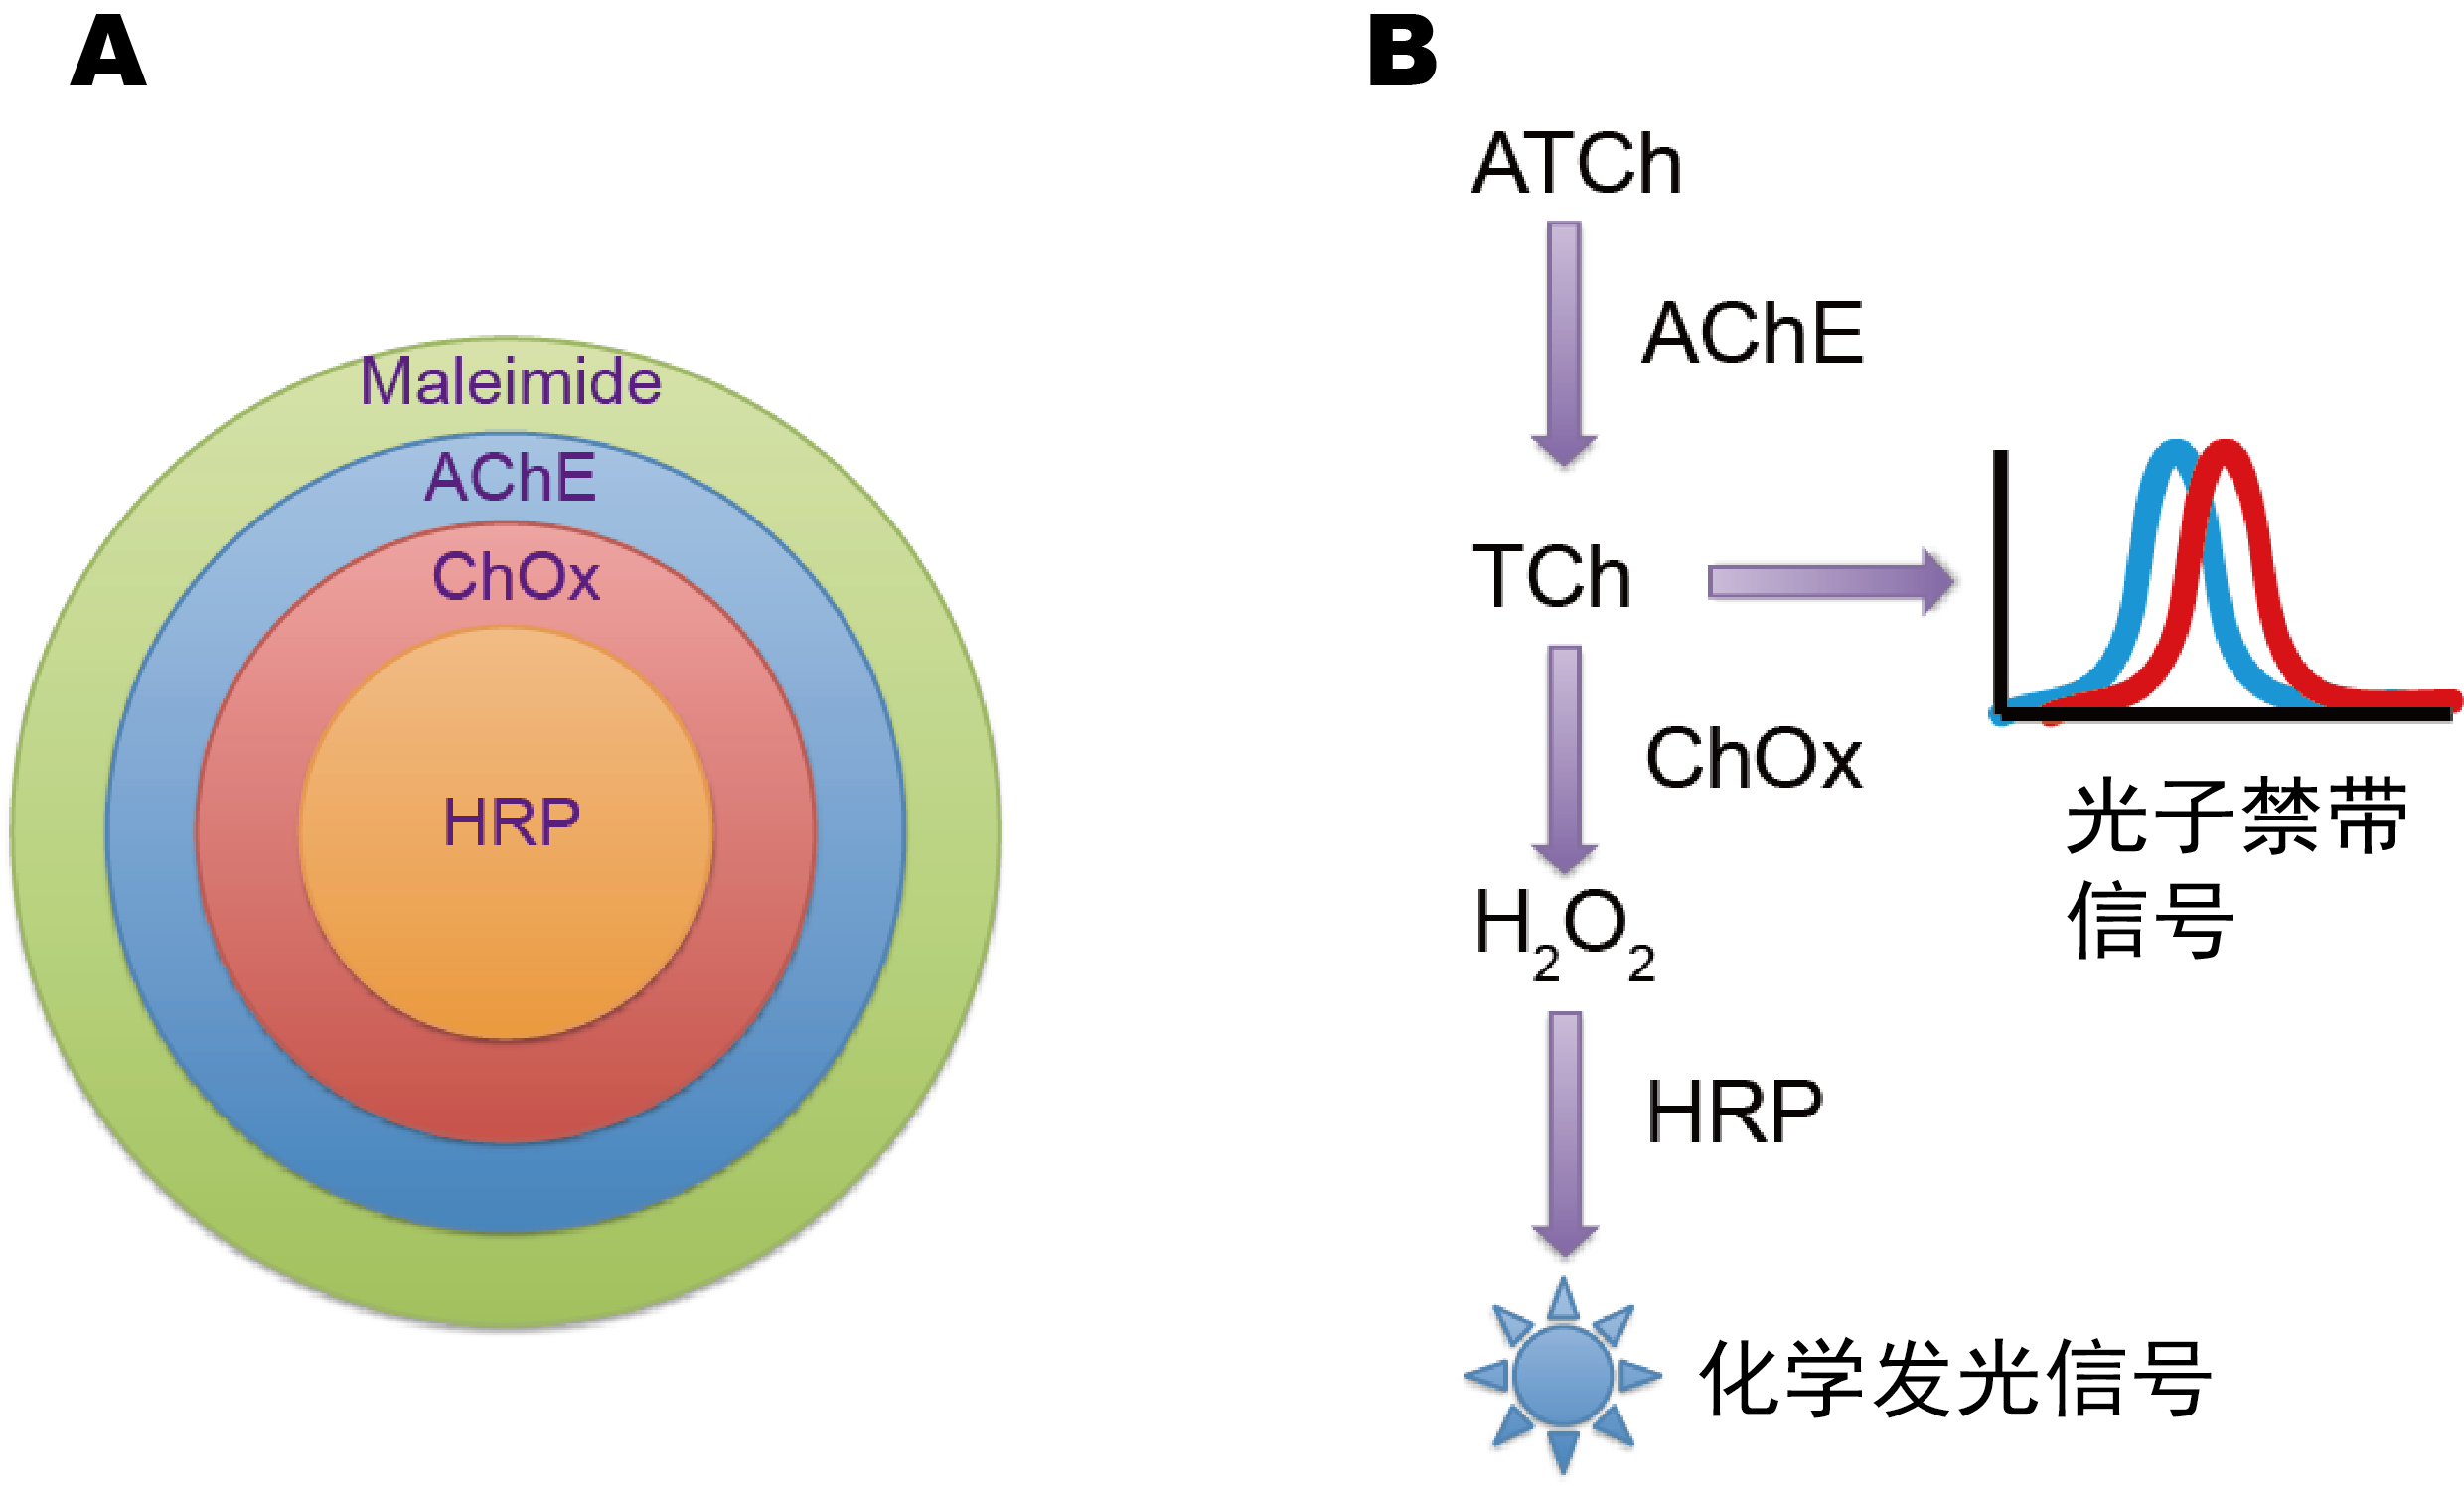
\includegraphics[width=0.7\linewidth]{figures/ch5/cascade-principle.png}
  \caption{本节中级联反应光子晶体微球的组成与信号表达原理。A. 光子晶体微球内部化学组成;B. 级联反应及信号表达原理图。}
  \label{fig:cascade-principle}
\end{figure}

首先,我们采用荧光标记的酶来对光子晶体微球进行标记。
如图~\ref{fig:cascade}A所示,不同的酶在光子晶体微球中接枝形成了互相独立的层状结构,说明这种刻蚀-反应方法同样适用于酶的接枝需求。
同时,我们对酶级联反应的信号表达进行了研究。
卢米诺的化学发光显示出级联反应在最内层的HRP处终止,由于酶的空间特异性修饰,使得化学发光产生的区域与HRP所在区域相重叠。此外,由于光子晶体内部的联通孔道结构,使得随着时间增长在中心化学发光强度增强的情况下,也存在一定的扩散(图~\ref{fig:cascade}B)。
\begin{figure}[htbp]
  \centering
  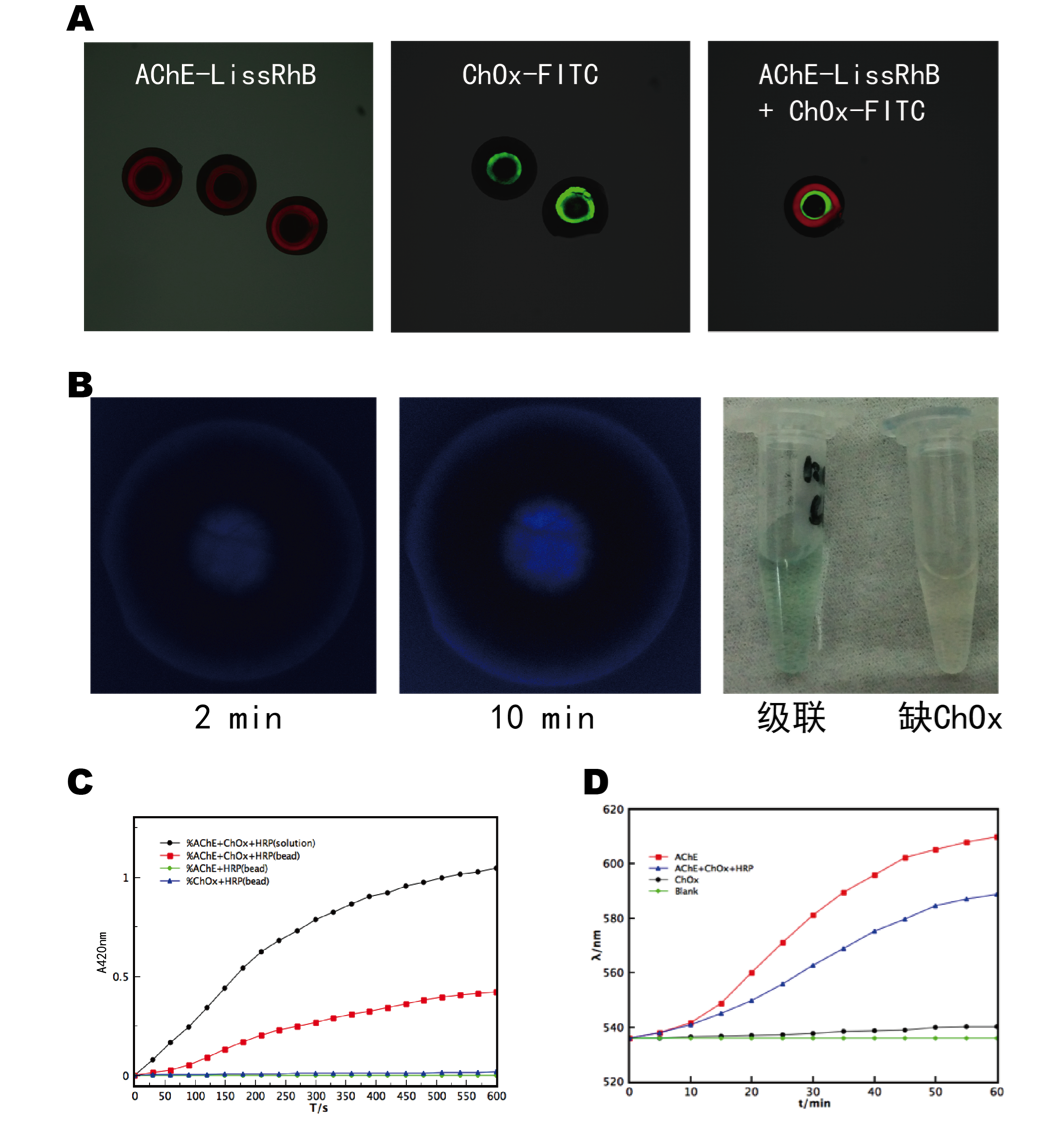
\includegraphics[width=\linewidth]{figures/ch5/cascade.png}
  \caption{光子晶体微球中级联反应及其表征。A. 荧光标记酶在光子晶体中定向修饰;B. 级联反应的化学发光及紫外可见吸收的响应;C. 不同酶组合条件下的级联反应的紫外可见吸收表征;D. 不同酶组合条件下的级联反应的光子晶体信号表达;}
  \label{fig:cascade}
\end{figure}

相对地,我们也利用ABTS的化学吸收吸收变化来研究光子晶体微球中的级联反应。由于ABTS氧化后在420 nm处产生新吸收峰,可以通过测定其420 nm的吸光度来反应级联反应进行的程度。
当级联反应链完整时,ABTS的吸光度随着时间而呈现增长,直观体现为形成绿色的氧化产物,而若级联反应链不完整时,几乎不能观察到ABTS吸光度的变化,证明了级联反应的完整性对与此体系的重要性。
此外我们可以注意到在光子晶体微球中发生的级联反应较同样浓度(按修饰酶的浓度计算)的液相反应体系略有降低(图~\ref{fig:cascade}C),这可能来自于接枝效率与刻蚀过程中对酶活性的影响,但总体来说采用HF/NH\text{$_4$}缓冲溶液进行刻蚀并不至于使酶失活。

最后,我们研究了酶反应对光子禁带的影响(图~\ref{fig:cascade}D)。与此前含马来酰亚胺的平面型光子晶体相似,AChE的水解产物TCh能够产生外层光子禁带的变化。即使光子晶体微球中只修饰了AChE,级联反应并不完整,但仍然能够显示出光子禁带的变化。而缺乏AChE的光子晶体微球则几乎没有光子禁带信号变化。此外,我们注意到多重酶接枝后的光子晶体微球的Bragg衍射峰增长速率满于单纯AChE接枝的光子晶体,间接说明了刻蚀过程中对酶活性的轻微影响。光子禁带的变化速率较化学发光法的速率略满,这来自于两方面原因:首先AChE的反应产物除了向外扩散形成光子禁带变化以外,很大一部分在级联反应中被消耗;其次,尽管有反蛋白石孔道促进化学反应,在聚合物上的化学反应仍慢于溶液相中的反应。

综上,我们利用刻蚀-反应法制备了具有级联反应特性的光子晶体微球。通过缓冲溶液的刻蚀,我们能够实现在光子晶体微球中的区域特异性生物酶的修饰,并且形成的功能区域互相独立。而利用酶的级联反应与双信号表达的特性,这种光子晶体微球材料能够很好地模拟实际细胞中的化学反应。更为重要的是,空间特异性的酶固定技术在生物工程、异相催化、以及生物模型研究中具有重要意义。
前这种酶的特异性接枝几乎都是由自下而上的方法制备得到\cite{Umler2010Coupled,Chandrawati2011Multicompartment},而本节中首次利用自上而下的修饰方法实现了空间特异性的酶接枝。结合多层结构的相互作用、光子晶体光学性质、反蛋白石孔道结构以及空间上的化学复杂度,我们希望这种光子晶体材料能够延伸发展为其他功能体系。


\section{本章小结}
本章中基于选择性刻蚀-反应成功实现了在光子晶体微球上的三维化学修饰与功能化。
所形成的多层光子晶体结构具有可调节的层数、组分及比例,且能够形成空间上的化学复杂度。
而光子晶体光学特性、孔道特性与三维复杂化学组成的有机整合使光子晶体具有极大的拓展性。
在这种光子晶体微球平台上,基于选择性刻蚀-反应实现了三维尺度上的亲疏水梯度、正交化学反应微球、自表达级联反应体系等应用。
展示了结构、化学组成各向异性的光子晶体微球在复杂功能体系中的潜在应用。
相信这种光子晶体微球平台的多功能整合能够进一步发展其他新颖的多功能体系,并且这种自上而下的光子晶体修饰方法能为微纳尺度材料的复杂修饰提供新的思路。
